\section{Introduction} \label{sec:intro}
This  course is aimed at introducing computer scientists to uses of computers and computational techniques in other areas of science.    The number of ways that computers are used in the sciences are many, varied and often extremely sophisticated.   The focus of this course will be  on  ``computational science'' which involves constructing mathematical models that can be simulated, analysed and solved using computational methods.  

The course is split into two parts:  in the first 3-4 weeks, we'll look at techniques for finding the roots of equations, solving systems of linear equations and decomposing matrices.  These techniques are basic to areas of research known as computational engineering, numerical analysis and applied linear algebra.  

In the remaining 8-9 weeks, we'll turn to computational biology, with a focus on bioinformatics and phylogenetics.  There, we see how a wide range of computational and mathematical techniques have revolutionised an area of science and allowed us to  analyse and interpret huge amounts of genetic data. This area of study has helped us better understand, among other things,  the basic workings of life,  our evolutionary  history, the causes of inherited diseases and the spread of infectious disease. 

From a computational point of view, computational biology is a fascinating and active area of research.  The techniques we'll study in this part of the course include stochastic and probabilistic modelling,  simulation, dynamic programming, estimation and inference.

CS 369 is more mathematical than many CS courses. This is unavoidable given the subject matter.   We assume that students have some background in discrete mathematics (matrices, graphs, linear equations) and continuous mathematics (functions, derivatives, integration), and an understanding of basic probability (discrete and continuous random variables, expectation, conditional probability) .    However, we recognise that students come to this course from a variety of  backgrounds so will provide explanations from quite a basic level in most cases.  We do assume that students have a solid foundation in programming in one of Java, C++, Python, Matlab or R.





\section{Mathematical modelling and why we need computers}
\label{sec:why}
Mathematical models attempt to precisely describe a system in order to better understand it.  A model is usually based on observing the system and is often structured to answer a particular question. It is not an exact replica of the system and is not merely a description of the observations.  Recorded observations of the system are known as data.   Coupled with data, the model allows us to infer unobserved properties of the model (such as model parameters) and predict future outcomes.  Careful comparison of outcomes predicted by the model with data (actual outcomes) tell us how accurate the model is and where it needs to be refined.


This process of modelling and observation has, arguably, been used for thousands of years and certainly for hundreds.  The complexity of the models we create and study is somewhat determined by our ability to interpret and ``solve'' them.  Before computers, we were largely limited to using models that were analytically tractable --- that is, models for which closed form  solutions could be found  --- or for which good approximations could be made by hand.  Our ability to fit models to data was severely  limited by our human limitations of collecting, storing and processing information by hand.  

With the advent of computers, both of these limitations have eased considerably.  It is now possible to collect and store massive amounts of data.  For example, Genbank, which stores genetic nucleotide sequences  contains over 204 billion nucleotide bases in more than 189 million sequences as at the end of 2015, while CERN's Large Hadron Collider produces 30 PB ($=30 \times 10^6$ GB) of data annually.  And fast computers allow us process this data and  to make  almost  arbitrarily good approximations to models that are far more complex than could be tackled by hand.  

However, even with all the data and computing power in the world we need to be careful to propose useful models  and tackle them with efficient techniques if we are to make progress in answering questions that interest us.  Bad models, bad data or bad computational techniques could all derail our quest for understanding.  In this course, we aim to teach good computational techniques and give some insight into some basic modelling and data analysis techniques that will help to tackle and answer a range of interesting questions.

\subsection{Why we need to be clever about our computing}

Mathematical problems can be classed into problems that are {\em well-posed} and {\em ill-posed}.  A problem is {\em well-posed} if 
\begin{enumerate}
\item A solution exists
\item the solution is unique
\item A small change in the initial condition induces only a small change in the solution
\end{enumerate}
A problem that is not well-posed is ill-posed.

We are interested in the last criterion which can be termed {\em sensitivity}.  Suppose our problem has inputs $x$ and has a solution (or output) $y$.  An {\em insensitive} or {well-conditioned} problem is when a change in $x$ causes a change in $y$ that is of similar relative size.  A {\em sensitive} or {\em ill-conditioned} problem is one in which the change in solution/output can be  large relative the the change in input.  

Based on this idea, define the {\em condition number} by 
\[ cond = \frac{|\mbox{relative change in solution}|}{|\mbox{relative change in input data}|} = \left|\frac{\Delta y/y}{\Delta x/x}\right |. \]
Thus a problem is {\em ill-conditioned} is $cond \gg 1.$

{\bf Example}:  what is the condition number when we evaluate a function $y = f(x)$ at an approximation of $x$, $\hat x = x+ \Delta x$, rather than at the true value $x$?

{\bf Solution}: \[ cond = \left|\frac{\Delta y/y}{\Delta x/x}\right | = \left|\frac{f(x+\Delta x) - f(x)/f(x)}{\Delta x/x}\right | = \left|\frac{f(x+\Delta x) - f(x)}{\Delta x} \frac {x}{f(x)}\right | \approx \left | \frac{x f'(x)}{f(x)} \right |.  \]
So, depending on the function $f$ and the input $x$, we could get very large condition numbers. \sqend

{\bf Example}:  What is the condition number for the functions $f(x) = x^n$ and $f(x) = e^x$?

{\bf Solution}: From above, the condition number is \[ cond \approx \left | \frac{x f'(x)}{f(x)} \right |. \]  When $f(x) = x^n$, $f'(x) = n x^{n-1}$, so  \[ cond =  \left | \frac{x f'(x)}{f(x)} \right | = \left | \frac{x . n x^{n-1}}{x^n} \right | = \left | \frac{ n x^{n}}{x^n} \right |  = |n|.\]
So as the degree of the polynomial increases, the problem becomes increasingly ill-conditioned.


Similarly, when $f(x) = e^x$, $f'(x) = e^x$ so \[ cond =  \left | \frac{x f'(x)}{f(x)} \right | = \left | \frac{x .e^x}{e^x} \right |  = |x|.\]
In this case, the condition number depends on the input argument, $x$.  If $x$ is very large, the problem can be considered ill-conditioned.   \sqend




What does this mean for computation?  In nearly all our computations, we will replace  exact formulations with approximations.  For example,  we approximate continuous quantities with discrete quantities, we are limited in size by floating point representation of numbers which often necessitates rounding or truncation and introduces (hopefully) small errors.  If we are not careful, these error will be amplified within an ill-conditioned problem an produce inaccurate results.

This leads us to consider the {\em stability}   and {\em accuracy} of our algorithms.   

An algorithm is {\em stable} if the result is relatively unaffected by perturbations during computation.  This is similar to the idea of conditioning of problems.  

An algorithm is {\em accurate} is the competed solution is close to the true solution of the problem.  Note that a stable algorithm could be inaccurate. 

We seek to design and apply stable and accurate algorithms to find accurate solutions to well-posed problems (or to find ways of transforming or approximating ill-posed problems by well-posed ones).



\section{Approximating a function by a Taylor series}

First, a little notation.  A real-valued function  $f:\mathbb R \to \mathbb R$ is a function  $f$ that  takes a real number argument, $x  \in \mathbb R$ ,and returns a real number, $f(x) \in \mathbb R$. We write $f'(x)$ to denote the derivative of $f$, so $f'(x) = \frac {df}{dx}$, and $f''(x)$ is the second derivative (so  $f'(x) = \frac{d}{dx}(\frac {df}{dx}) = \frac{d^2 f}{dx^2}$) and $f^{(k)}(x)$ is the $k$th derivative of $f$ evaluated at $x$.

As we have just seen, simply evaluating a real valued function can be prone to instability (if the function has a large condition number).  For that reason, approximations of functions are often used.   The most common method of approximating the real-valued function $f:\mathbb R \to \mathbb R$  by a simpler function is to use the Taylor series representation for $f$.  

The Taylor series has the form of a polynomial where the coefficients of the polynomial are the derivatives of $f$ evaluated at a point. So long as all  derivatives of the function exists at the point $x = a$, $f(x)$ can be expressed in terms of of the value of the function and it's derivatives at $a$ as:
\[ f(x) = f(a) + (x-a)f'(a) + \frac{(x-a)^2}{2!}f''(a) + \ldots + \frac{(x-a)^k}{k!}f^{(k)}(a) + \ldots \]
This can be written more compactly as 
\[ f(x) = \sum_{k = 0}^{\infty} \frac{(x-a)^k}{k!}f^{(k)}(a), \]
where $f^{(0)} = f$ and $0! = 1$ by definition.  

This is known as the {\em Taylor series} for $f$ about $a$.  It is valid for $x$ ``close'' to $a$ (strictly, within the ``radius of convergence'' of the series).   When $a = 0$, the Taylor series  is known as a {\em Maclaurin series}.

This is an infinite series (the sum contains infinitely many terms) so cannot be directly computed.  In practice, we truncate the series after $n$ terms to get  the {\em Taylor polynomial of degree $n$} centred at $a$, which we denote $\hat f_n(x;a)$:
\[ f(x) \approx \hat f_n(x;a) = \sum_{k = 0}^{n} \frac{(x-a)^k}{k!}f^{(k)}(a). \]
This is an approximation of $f$ that can be readily calculated so long as the first $n$ derivatives of $f$ evaluated at $a$ can be calculated.  The approximation can be made arbitrarily accurate by increasing $n$.  The quality of the approximation also depends on the distance of $x$ from $a$ --- the closer $x$ is to $a$, the better the approximation.

{\bf Example}: Find the Taylor approximation of $f(x)=\exp(x) =  {e}^x$ for values of  $x$ close to 0. 

{\bf Solution:} The $k$th derivative of  $f(x) = e^x$ is simply $e^x$ for all $k$.  Since we want values of $x$ close to 0, find the Taylor series about  $a = 0$ (the Maclaurin series).   Then 
 
\[ \widehat{f}_n(x;0) = 1 + \frac{x}{1!} + \frac{x^2}{2!} + \frac{x^3}{3!} + \cdots = \sum\limits_{k=0}^{n}\frac{x^k}{k!} \]

 This  series converges to $\mathrm{e}^x$ everywhere: $\lim\limits_{\rightarrow\infty} \widehat{e}_n(x)= e^x$.  The quality of the approximation for various values of $n$ and $x$ are studied in the table below.
\[
\begin{array}{r|ccccc|c}
n & 1 & 2 & 3 & 4 & \ldots & \textsf{true value }e^x\\ \hline
\widehat{f}_n(x=1;0) & 2.0000 & 2.5000 & 2.6667 & 2.7083 & \ldots & {2.7183}\\
\textsf{\scriptsize Relative error} & 0.26 & 0.08 & 0.019 &  0.0037 & &\\ \hline\hline
\widehat{f}_n(x=2;0) & 3.0000 & 5.0000 & 6.3333 & 7.0000 & \ldots  & {7.3891}\\
\textsf{\scriptsize Relative error} & 0.59 & 0.32 & 0.14 &  0.053 & &\\ \hline
\end{array}
\]

Notice that the error is smaller for $x$ close to $a$ and decreases as $n$, the number of terms in the polynomial increases.   \sqend


\section{Finding the roots of equations}

Given a real valued function $f:\mathbb R \to \mathbb R$,  a fundamental problem is to find the values of $x$ for which $f(x) = 0$.  This is known as finding the roots of $f$.  The problem crops up again and again and many problems can be reformulated as this problem.  For example, if the trajectory of one object is described by $h(x)$, while another object has trajectory $g(x)$, then the two objects intercept one another exactly when $f(x) = g(x) - h(x) = 0. $

Another common application is when we wish to find the minimum or maximum value that a function takes.  We know from basic calculus that if $f$ is the derivative of some function $F$, then $F(x)$ takes its  maximum or minimum values when $f(x) = 0$.  Thus finding the maximum value of $F$ is a matter of finding the roots of $f$.  

We will consider two simple yet effective root finding algorithms.  The bisection method and Newton's method.  In both cases, we assume that $f:\mathbb R \to \mathbb R$ is continuous.

\subsection{Bisection method}

We want to find $x^*$ such that $f(x^*) = 0$.  Let $\mathrm{sign}(f(x)) = -1$ if $f(x) < 0$ and $\mathrm{sign}(f(x)) = 1$ if $f(x) > 0$.  The bisection method proceeds as follows:

\begin{itemize}
\item {\bf Initialise:} Choose initial guesses $a, b$ such that $\mathrm{sign} f(a) \ne\mathrm{sign} f(b)$
\item {\bf Iterate} until the absolute difference $ |a-b| \approx 0$
\begin{itemize} 
\item Calculate $c=\frac{a+b}{2}$
\item If $\mathrm{sign} f(a) =\mathrm{sign} f(c)$, then $a\leftarrow c$; otherwise $b\leftarrow c$
\end{itemize}
\end{itemize}

The method provides slow but sure convergence.
\begin{figure}[htbp]
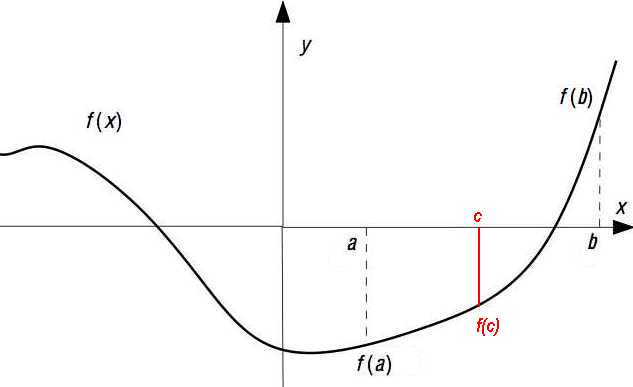
\includegraphics[width=4in]{figures/bisectionIdea.jpg}
\caption{The idea behind the bisection method. Here, $\mathrm{sign} f(a) =\mathrm{sign} f(c)$ so at the next iteration we will set $a \leftarrow c$. The algorithm stops when $a$ and $b$ are sufficiently close to each other.}
\end{figure}

\subsection{Newton's method}

This method is also known as the Newton-Raphson method and is based on the approximation first two terms of the Taylor series expansion.  Recall that we want to find $x$ such that $f(x) = 0$. From the first two terms of the  Taylor series of $f(x)$, we know that  $f(x)  \approx f(a) + (x - a) f'(a)$.  If $f(x)$ is zero, then the expression on the right hand side to 0 and solve for $x$ to get  
\[ f(a) + (x - a) f'(a) = 0 \implies  x = a - \frac{f(a)}{f'(a) }.\]
We can treat this iteratively, starting at $x_0$, and finding $x_{i+1} = x_i - \frac{f(x_i)}{f'(x_i) }$.  This leads to the algorithm:
\begin{itemize}
\item {\bf Initialise:} Choose $x_0$ as an initial guess.
\item {\bf Iterate} until the absolute difference $\vert x_i-x_{i-1} \vert \approx 0$
\begin{itemize} 
\item Set $x_{i+1} = x_i - \frac{f(x_i)}{f'(x_i) }.$
\end{itemize}
\end{itemize}

{\bf Example}: $f(x) = x^2 - 2$.

{\bf Solution}:  $f'(x) = 2x$ so 
\[
x_{i+1} =  x_i - \frac{f(x_i)}{f'(x_i) } = x_i - \frac{x_i^2 - 2}{2x_i} = \frac{x_i}2 + \frac1{x_i}.
 \]
See slide for example starting at $x_0 = 0.5$. \sqend


Compare with bisection method: Start at $a = 1/2$ and $b = 2$ to get to $a = 1.34375$ and $b = 1.4375$ at the fifth step.  This produces an absolute error of $0.02688$ or 1.9\%.  The absolute error in the Newton case is 0.00020 which is 2 orders of magnitude smaller.

\begin{figure}[htbp]
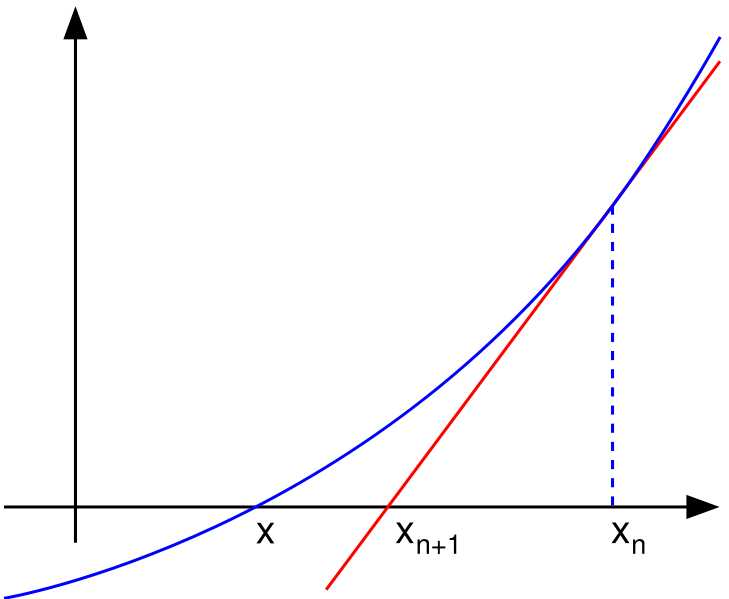
\includegraphics[width=4in]{figures/NewtonIteration.jpg}
\caption{The idea behind the Newton's method. Starting at $x_n$, we find the tangent line (red) and calculate the point it intercepts the $x$-axis.  This point of intercept is $x_{n+1}$.  }
\end{figure}

%%\notinexam{
There are, of course, many other root finding methods.  We list a few of them here (not examinable).

 Secant method (\url{http://en.wikipedia.org/wiki/Secant\_method}):
\begin{itemize}\setlength{\itemsep}{0pt}
\item Newton's method with a finite difference instead of the derivative
\item Neither computation, nor existence of a derivative is required 
\item However, the convergence is slower (approximately, $\alpha=1.6$)
\end{itemize}
False position method (\url{http://en.wikipedia.org/wiki/False\_position\_method}):
\begin{itemize}\setlength{\itemsep}{0pt}
\item Always retains one point on either side of the root 
\item Faster than the bisection and more robust than the 
secant method
\end{itemize}
Muller's method  (\url{http://en.wikipedia.org/wiki/Muller's\_method}):
\begin{itemize}\setlength{\itemsep}{0pt}
\item Quadratic (instead of linear) interpolations
\item Faster convergence than with the secant method
\item Roots may be complex (in addition to reals)
\end{itemize}
%%}%end not in exam
\newpage

\section{Numerical linear algebra}

Numerical linear algebra is one of the cornerstones of modern mathematical modelling.  Topics as important as solving systems of ordinary differential equations (arising in engineering, economics, physics, biotech, etc),  to network analysis (telecoms, sociologic, epidemiology), internet search, data mining and many more rely on linear algebra.  

These days, applied linear algebra and numerical linear algebra are virtually interchangeable --- problems of all sizes are routinely solved numerically and rely on a wealth of mathematical and computational insight.  

We'll start out with a brief review of topics that you should be somewhat familiar with.


\subsection{Review}

Let $\mathbf{a}=\left[\begin{array}{c}a_1\\ \vdots \\ a_n\end{array}\right]$    
$\mathbf{b}=\left[\begin{array}{c}b_1\\ \vdots \\ b_n\end{array}\right]$ be vectors.  The {\em inner} or {\em dot product} of $\mathbf{a}$ and $\mathbf{b}$  is 
the scalar $c=\mathbf{a}\bullet\mathbf{b} \equiv \mathbf{a}^{\mathsf{T}}\mathbf{b} =\sum\limits_{i=1}^n a_i b_i$. 
The dot product is also called {\em multiplication} of vectors.

The {\em norm} or {\em magnitude} of a vector $\mathbf a$ is  $||\mathbf a|| = \sqrt{a \cdot a} =  \sqrt{\mathbf a^{\mathsf T} \mathbf a} = \sqrt{a_1^2 + \ldots a_n^2}$.

The {\em product} of an $m \times n$ {matrix} 
$\mathbf{A} = \left[ \begin{array}{ccc} A_{11}& \ldots & A_{1n}\\ \vdots &\ddots &\vdots \\ A_{m1}& \ldots &A_{mn} \end{array}\right]$
and an $n\times 1$ ($n$-dimensional) {vector} $\mathbf{x}=\left[\begin{array}{c}x_1\\\vdots\\x_n\end{array}\right]$ is
the $m$-dimensional vector $\mathbf{y}=\mathbf{Ax}$ with the elements $y_i=\sum\limits_{j=1}^m A_{ij}x_j$.

The {\em product} of a $k \times m$ matrix $\mathbf{A}$ and an $m \times n$ {matrix} $\mathbf{B}$ is
the $k \times n$ matrix $\mathbf{C}=\mathbf{AB}$ with the elements $C_{ij}= \sum\limits_{\alpha=1}^{m}A_{i,\alpha}B_{\alpha,j}$

The {\em outer product} of an $m$-dimensional  vector $\mathbf a$ with an $n$-dimensional vector $\mathbf b$ is the $m \times n$ matrix 
\[
\mathbf{a}\mathbf{b}^{\mathsf{T}}\equiv
\left[\begin{array}{c}a_1\\ a_2 \\ \vdots \\ a_m\end{array}\right]
\left[\begin{array}{cccc}b_1&b_2&\ldots&b_n\end{array}\right] =
\left[\begin{array}{cccc}a_1b_1 & a_1b_2 & \ldots & a_1b_n\\
                                          a_2b_1 & a_2b_2 & \ldots & a_2b_n\\
                                          \vdots    & \vdots     & \ddots & \vdots \\
                                          a_mb_1 & a_mb_2 & \ldots & a_mb_n
                                          \end{array}\right]
\] 

The {\em identity matrix} of size $n$, $\mathbf I_n$, is the $n \times n$ matrix with $(i,j)$th entry = 0 if $i \ne j$ and $1$ if $i = j$.  

The {\em inverse} of a square matrix $\mathbf A$ of size $n$ is the square matrix $\mathbf A^{-1}$ such that $\mathbf{AA}^{-1} = \mathbf I_n = \mathbf A^{-1}\mathbf A$. When such a matrix exists, $A$ is called {\em invertible} or {\em non-singular}. $\mathbf A$ is {\em singular} if no inverse exists.  Finding the inverse of $\mathbf  A$ is typically difficult.

The {\em determinant} of  an $n \times n$ matrix $\mathbf A$, written $det(\mathbf A) = \left| \begin{array}{ccc} A_{11}& \ldots & A_{1n}\\ \vdots &\ddots &\vdots \\ A_{n1}& \ldots &A_{nn} \end{array}\right|$, is given by a somewhat complex formula that we need not reproduce here (look it up at  \url{http://en.wikipedia.org/wiki/Determinant}).  For $n= 2$, $det(A)  = A_{11} A_{22} -  A_{21} A_{12}$.  For $n= 3$, $det(A)  = A_{11}A_{22}A_{33} - A_{31}A_{22}A_{13} + A_{12}A_{23}A_{31} - A_{32}A_{23}A_{11} + A_{13}A_{21}A_{32} - A_{33}A_{21}A_{12}$.

{\bf Example}: Find the determinant of $\mathbf  A = \left(\begin{array}{ll}3 & 5\\1&-1\end{array}\right) $.

{\bf Solution}: From above, $det(\mathbf A) = |\mathbf A| = 3 . {-1}  - 1.5 = {-3} -5 = -8$. \sqend

It is worth recalling a few properties of the determinant (as listed on the wiki page): 
\begin{itemize}
\item $det(\mathbf I) = 1$ 
\item $det(A^T) = det(A)$ (transposing the matrix does not affect the determinant) 
\item $det(A^{-1}) = \frac{1}{det(A)}$ (the determinant of the inverse is the inverse of the determinant)
\item For $A, B$ square matrices of equal size, $det(AB) = det(A)det(B)$
\item $det(cA) = c^n\, det(A)$ for any scalar $c$
\item If $A$ is triangular (so has all zeros in the upper or lower triangle) then $det(A) = \prod_{i = 1}^n A_{ii}$.
\end{itemize}


An {\em eigenvector} of the square matrix $\mathbf A$ is a non-zero vector $\mathbf e$ such that $\mathbf A \mathbf e = \lambda \mathbf e$ for some scalar $\lambda$.  $\lambda$ is known as the {\em eigenvalue} of  $\mathbf A$  corresponding to $\mathbf e$.  Note that $\lambda$ may be 0.   So the effect of multiplying $e$ by $A$ is simply to scale $e$ by the corresponding scalar $\lambda$.  

The determinant can be used to find the eigenvalues of $\mathbf A$:   they are the roots of
the {\em characteristic polynomial} $p(\lambda) = \det(\mathbf{A }- \lambda\mathbf{I}_n)$
where $\mathbf{I}_n$ is the identity matrix.


{\bf Example}: Find the eigenvalues of $\mathbf  A = \left(\begin{array}{ll}3 & 5\\1&-1\end{array}\right) $.

{\bf Solution}: We need to solve $p(\lambda) = \det(\mathbf{A }- \lambda\mathbf{I}_2) = 0$. 
\[ \begin{array} {lcl}  | \mathbf{A }- \lambda\mathbf{I}_2 |  &= &   \left\vert \left(\begin{array}{ll}3 & 5\\1&-1\end{array}\right) - \lambda  \left(\begin{array}{ll}1 & 0\\0&1\end{array}\right) \right\vert \\
& = &   \left\vert \begin{array}{ll}3-\lambda & 5\\1&-1 - \lambda\end{array}  \right\vert \\
& = & (3-\lambda)(-1 - \lambda) - 5  \\
& = &  - \lambda^2 -2\lambda  -8 \\
& = & (\lambda + 2 )(\lambda - 4 )
\end{array}
\]
which is zero when $\lambda = 4$ or $\lambda = -2$. So the eigenvalues of $\mathbf A$ are $\lambda = 4$ and $\lambda = -2$.  \sqend

%{\bf Example}: For a $2\times2$ matrix $\mathbf{A}$,
%\[
%\begin{array}{ll}
%& \mathrm{det}(\mathbf{A}-\lambda\mathbf{I}) \equiv\left\vert\begin{array}{ll}A_{11}-\lambda& A_{12}\\A_{21}&A_{22}-\lambda\end{array}\right\vert \\ \\
%{\Rightarrow} &
%p(\lambda) = \lambda^2 - \left(A_{11}+A_{22}\right)\lambda + A_{11}A_{22}-A_{12}A_{21} = 0.
%\end{array}
%\]

{\bf Example}: Find the eigenvector of $\mathbf  A = \left(\begin{array}{ll}3 & 5\\1&-1\end{array}\right) $ corresponding to the eigenvalue $\lambda = -2$.

{\bf Solution}: The eigenvector  $\mathbf e$ corresponding to $\lambda = -2$ satisfies the equation $\mathbf{Ae} = -2 \mathbf e$.  That is,
\[ \left(\begin{array}{ll}3 & 5\\1&-1\end{array}\right)  \left( \begin{array}{c} e_1 \\ e_2 \end{array}\right) = -2 \left( \begin{array}{c} e_1 \\ e_2 \end{array}\right).\]
This is the system of linear equations \begin{eqnarray}  3e_1 + 5e_2 &=& -2e_1, \\ e_1 - e_2 &=& -2 e_2. \label{eqn:eigenvec} \end{eqnarray}
Rearranging either equation, we get $e_1 = -e_2$, so both equations are the same.  We thus fix $e_1 = 1$ and the eigenvector associated with $\lambda = -2$ is $\mathbf e = \left( \begin{array}{c} 1 \\ -1 \end{array}\right)$.  Notice that the choice to fix  $e_1 = 1$ was arbitrary.  We could choose any value so, strictly, $\mathbf e =  c\left( \begin{array}{c} 1 \\ -1 \end{array}\right)$ for any $c \neq 0$.  Often, $c$ is chosen so that $\mathbf e$ is normalised (see below).  In this case, choose $c = 1/\sqrt 2$ to normalise $\mathbf e$. \sqend



Vectors $a$ and $b$ are {\em orthogonal} if the dot product $a^Tb = 0$.  Orthogonal generalises the of the idea of the perpendicular.  In particular, a set of vectors $\{ \mathbf e_1, \ldots, \mathbf e_n \}$ is {\em mutually orthogonal} if each pair of vectors $e_i, e_j$ is orthogonal for $i \ne j$.

A vector $\mathbf e_i$ is normalised if $\mathbf e_i^T e_i = 1$.

A set of vectors that is mutually orthogonal and has each vector normalise is called {\em orthonormal}. 


Any symmetric, square matrix $\mathbf A$ of size $n$ has exactly $n$ eigenvectors that are mutually orthogonal.


 

Any square matrix $A$ of size $n$ that has $n$ mutually orthogonal eigenvectors can be represented via the {\em eigenvector representation} as follows: 
\[
\mathbf{A} = \sum\limits_{i=1}^n \lambda_i\underbrace{\mathbf{e}_i\mathbf{e}_i^{\mathsf{T}}}_{\mathbf{U}_i}
\]
where $\mathbf{U}_i=\mathbf{e}_i\mathbf{e}_i^{\mathsf{T}}$ is an $n\times n$ matrix.


The {\em Range}, $\mathrm{range}(\mathbf{A})$, or span of an $m\times n$ matrix $\mathbf{A}$ 
is  the set of vectors $\mathbf{y}\in\mathbb{R}^m$ such that $\mathbf{y}=\mathbf{A}\mathbf{x}$ for some $\mathbf{x}\in\mathbb{R}^n$.  The range is also referred to as the {\em column space} of  $\mathbf{A}$ as it is the space of all linear combinations of the columns of $\mathbf{A}$.


The {\em Nullspace}, $\mathrm{null}(\mathbf{A})$, of an $m\times n$ matrix $\mathbf{A}$
is the set of vectors $\mathbf{x}\in\mathbb{R}^n$, such that $\mathbf{A}\mathbf{x}=\mathbf{0}\in\mathbb{R}^m$ 

The {\em Rank}, $\mathrm{rank}(\mathbf{A})$, of an $m\times n$ matrix $\mathbf{A}$ is the dimension of the range of $\mathbf{A}$ or of the column space of $\mathbf{A}$.  $\mathrm{rank}(\mathbf{A}) \leq \min\{m,n\}$.

\newpage

\subsection{Review of eigenvectors and eigenvalues}

\begin{itemize}
\item $\lambda$ is an eigenvalue of $\mathbf{A}$ if determinant $\vert\mathbf{A}-\lambda\mathbf{I}\vert=0$
\item This determinant is a polynomial in $\lambda$ of degree $n$:  so it has 
$n$ roots $\lambda_1,\lambda_2,\ldots,\lambda_n$
\item Every {symmetric} matrix $\mathbf{A}$ has a full set ({basis}) of $n$ orthogonal unit eigenvectors
$\mathbf{e}_1,\mathbf{e}_2,\ldots,\mathbf{e}_n$
\end{itemize}

\begin{itemize}
\item No algebraic formula for the polynomial roots for $n > 4$ 
\begin{itemize}
\item Thus, the eigenvalue problem needs own special algorithms
\item Solving the eigenvalue problem is harder than solving $\mathbf{Ax} = \mathbf{b}$
\end{itemize}
\item Determinant
 $\vert\mathbf{A}\vert = \prod_{i = 1}^n \lambda_i =  \lambda_1\lambda_2\cdots\lambda_n$ (the product of eigenvalues)
\item The {\em trace} of a matrix is the sum of the diagonal elements.  That is, \\ $\mathrm{trace}(\mathbf{A}) = \sum_{i=1}^n a_{ii} = a_{11}+a_{22}+\ldots+a_{nn}$.  
\item It turns out that $\mathrm{trace}(\mathbf{A}) = \sum_{i = 1}^n \lambda_i
            = \lambda_1+\lambda_2+\ldots+\lambda_n$ (the sum of eigenvalues)
 \item $\mathbf{A}^k= \underbrace{\mathbf{A}\cdots\mathbf{A}}_{k\textsf{  times}}$ has the same eigenvectors as $\mathbf{A}$: 
 e.g. for $\mathbf{A}^2$\vspace*{-3mm}
 \[
 \mathbf{A}\mathbf{e} = \lambda\mathbf{e} \;\; {\Rightarrow}\;\;\mathbf{A}\mathbf{A}\mathbf{e} = \lambda\mathbf{A}\mathbf{e} = \lambda^2\mathbf{e}
 \]\vspace*{-3mm}
\item Eigenvalues of $\mathbf{A}^k $ are $\lambda_1^k,\ldots, \lambda_n^k$
\item Eigenvalues of $\mathbf{A}^{-1}$ are 
 $\frac{1}{\lambda_1},\ldots,\frac{1}{\lambda_n}$
\end{itemize}
 
{\bf Example}: Find the eigenvalues and eigenvectors of $\mathbf{A} = \left[\begin{array}{rr}2 & -1\\-1 & 2\end{array}\right]$

{\bf Solution:} First, find the eigenvalues of $\mathbf A$ by solving 
\[
\vert\mathbf{A}-\lambda\mathbf{I}\vert=
\left\vert\begin{array}{rr}2-\lambda & -1\\-1 & 2-\lambda \end{array}\right\vert = 
\lambda^2 - 4\lambda +3 = (\lambda - 1)(\lambda -3) = 0.
\]
So the eigenvalues are $ \lambda_1 = 1 \mbox{ and } \lambda_2 = 3$

The eigenvector associated with $\lambda_1 = 1$ is $\mathbf e_1$ and satisfies $\mathbf {Ae}_1 = \lambda _1 \mathbf e_1$.  Putting $\mathbf{e}_1=\left[\begin{array}{r} x_1 \\ y_1 \end{array}\right]$ we need to solve 
\[ \left[\begin{array}{rr}2 & -1\\-1 & 2\end{array}\right]\left[\begin{array}{r} x_1 \\ y_1 \end{array}\right] = \left[\begin{array}{r} x_1 \\ y_1 \end{array}\right]. \]
 The second row gives $-x_1 + 2y_1 = y_1$, so $y_1 = x_1$.  So fix $x_1 = 1$ and $e_1 = c\left[\begin{array}{r} 1 \\ 1 \end{array}\right]$ for any $c \neq 0$.  If we choose $c$ so that $e_1$ is normalised,  $ \mathbf{e}_1=\frac{1}{\sqrt{2}}\left[\begin{array}{r} 1 \\ 1 \end{array}\right]$.  
 A similar argument shows $\mathbf{e}_2=\frac{1}{\sqrt{2}}\left[\begin{array}{r} 1 \\ -1 \end{array}\right] $.


Before leaving this example, it is worth looking at some of the properties of the eigenvalues of $\mathbf A$:
\begin{itemize}
\item Determinant $\mathrm{det}\ \mathbf{A}\equiv|\mathbf{A}|=4-1 = 3 \Longleftrightarrow \lambda_1\cdot\lambda_2 \equiv 1\cdot 3 = 3$
\item $\mathrm{trace}(\mathbf{A}) = 2 + 2 = 4 \Longleftrightarrow \lambda_1 + \lambda_2 \equiv 1 + 3 = 4$
\item Inverse matrix $\mathbf{A}^{-1}=\frac{1}{3}\left[\begin{array}{rr}2 & 1\\1 & 2\end{array}\right]$: eigenvalues 
$\lambda_1=\frac{1}{3}$  and $\lambda_2=1$
\item Matrix $\mathbf{A}^2 =  \left[\begin{array}{rr}5 & -4\\-4 & 5\end{array}\right]$: eigenvalues 
$\lambda_1=1$  and $\lambda_2=9$
\item Matrix $\mathbf{A}^3 =  \left[\begin{array}{rr}14 & -13\\-13 & 14\end{array}\right]$: eigenvalues 
$\lambda_1=1$  and $\lambda_2=27$
\end{itemize} \sqend




\subsection{Review of systems of linear equations}

A linear equation in $n$ unknowns $x_1, \ldots, x_n$ is of the form $a_1x_1 + \ldots a_nx_n = b$.  Given $m$ such equations, we can write the $i$th equation as $a_{i1}x_1 + \ldots a_{in}x_n = b_i$.  We will seek to solve these systems of linear equations.

{\bf Example} a system of 3 equations in 3 unknowns and its solution is 
\[ \left\{\begin{array}{rrrrrrr}
4x_1 &  + &  x_2  & + & 2x_3 & = & 24\\
2x_1 & - & x_2 & -  & 2x_3 & = & -6 \\
-x_1 & + & 2x_2 & - & x_3 & = & -4
\end{array}\right. {\Longrightarrow} \left\{\begin{array}{r}x_1=3\\x_2=2\\x_3=5\end{array}\right.\] \sqend

These systems can be represented as a matrix equation $\mathbf{Ax} = \mathbf b$ where $\mathbf A$ is the $m \times n$ matrix of coefficients, $a_{ij}$, $\mathbf{x}=\left[\begin{array}{c}x_1\\\vdots\\x_n\end{array}\right]$ is the $n$-dimensional column vector of unknowns and $\mathbf b$ is a vector of dimension $m$.

{\bf Example cont.} In the example above, $\mathbf A = \left[\begin{array}{rrr}4&1&2\\ 2 &-1& -2\\ -1 & 2 & -1\end{array}\right]$ and $\mathbf b = \left[\begin{array}{r}24 \\ -6 \\-4\end{array}\right]$ \sqend

We'll initially look at systems of $n$ equations and $n$ unknowns.  Systems  with $m < n$ are known as {\em under-determined} as there are less equations than unknowns while systems with $m > n$ are {\em over-determined} with more equations than there are unknowns.

When $A$ is non-singular (so $A^{-1}$ exists), the system has a unique solution given by $\mathbf x = \mathbf A^{-1}\mathbf b$.

 Recall that $\mathbf{A}$ is  nonsingular if and only if:\\ 
\hspace*{33mm} ({\em i})  inverse matrix $\mathbf{A}^{-1}$ exists; or \\
\hspace*{33mm} ({\em ii}) $\mathrm{det}(\mathbf{A})\ne 0$; or\\
\hspace*{33mm} ({\em iii})  $\mathrm{rank}(\mathbf{A})=m$, or \\
\hspace*{33mm} ({\em iv}) $\mathbf{Ax}\ne\mathbf{0}$ for any vector $\mathbf{x}\ne \mathbf{0}$, or\\
\hspace*{33mm} ({\em v}) $\mathrm{range}(\mathbf{A}) = \mathbb{R}^m$, or \\
\hspace*{33mm} ({\em vi}) $\mathrm{null}(\mathbf{A})=\{\mathbf{0}\}$.

If $\mathbf A$ is singular, the system may have infinitely many solutions or no solutions at all, depending on $\mathbf b$.

{\bf Example} If $\mathbf A = \left[\begin{array}{rr}2&3\\4&6\end{array}\right]$, $\mathbf{Ax} = \mathbf b$ has no solution if $\mathbf b \notin \mathrm{range}(\mathbf{A})$ or infinitely  many solutions when $\mathbf b \in \mathrm{range}(\mathbf{A})$.  Thus, when $\mathbf b = \left[\begin{array}{r}4\\7\end{array}\right]$ there is no solution, while when $\mathbf b = \left[\begin{array}{r}4\\8\end{array}\right]$, $\mathbf{x}=\left[ \begin{array}{c}\gamma\\\frac{2}{3}(2-\gamma)\end{array}\right]$ is a solution for any real $\gamma$. \sqend


\section{Solving linear equations}

In principle, all we need to do to solve the system of equations $\mathbf {Ax} = \mathbf b$ is find the inverse of $\mathbf A$, $\mathbf A^{-1}$.  Then $ \mathbf {Ax} = \mathbf b \implies \mathbf {A^{-1}Ax}  = \mathbf {A^{-1}b}  \implies \mathbf x = \mathbf  {A^{-1}b}$.  In practice, however, things are more complicated.  First, $\mathbf A$ only has an inverse if it is square (so $m = n$) and $det(A) \ne 0$.  In most cases, $m \ne n$ and often even when $m = n$,  $det(A) = 0$ is not unusual.  Second, supposing that $A$ is indeed square, $m$ and $n$ are often large ($10^4$ is common, as are much larger values).  In these cases, even calculating $det(A)$ is a hugely expensive and complex computational task while finding $\mathbf A^{-1}$ is even harder.

We'll initially concentrate on easily solvable systems and look at how we can coerce other systems into a form where they (or some close approximation) too are easily solvable. 

\subsection{Easily solvable systems 1: Diagonal matrix}

All the simple systems we consider here are assumed to be square, so $m = n$.  We want to solve $\mathbf {Ax} =\mathbf b$.

$\mathbf A$ is {\em diagonal} all entries the off-diagonal are zero.  That is $a_{ij} = 0$ when $i \ne j$.   So to specify a diagonal matrix, we need only specify the $n$ diagonal elements.  We can thus use the simplifying notation, $\mathbf{A}=\mathrm{diag}\{a_1,\ldots,a_n\}$.

When $A$ is diagonal, $x_i = \frac{b_i}{a_i}$ for all $i=1,\ldots, n$.  That is, $\mathbf A^{-1} = \mathrm{diag}\{\frac 1 {a_1},
\ldots, \frac1 {a_n} \}$. Or, to use less compact notation:
\[
\mathbf{A} = \left[       
\begin{array}{lll}
 a_{1}  & & \\ & \ddots & \\ & & a_n
\end{array}
\right] \; \Rightarrow \; \mathbf{A}^{-1} = \left[       
\begin{array}{lll}
 \frac{1}{a_{1}} & &\\ & \ddots & \\ & & \frac{1}{a_n}
\end{array}
 \right].
\]

\subsection{Easily solvable systems 2: Triangular matrix}

A matrix is {\em lower triangular} when all entries above the main diagonal are 0.  That is, $\bf A$ is lower triangular if and only if $a_{ij} = 0$ when $i < j$.  Similarly, a matrix is {\em upper triangular} when all entries above the main diagonal are 0 ($a_{ij} = 0 $ for $i > j$).  Lower triangular is also called left triangular, and upper called right triangular, for obvious reasons.  
E.g., a lower triangular matrix:
\[
\mathbf{A}=\left[
\begin{array}{llll}
a_{11} &       0       &     \ldots        &                0\\
a_{21} & a_{22} &        \ddots        &       \vdots        \\
\vdots  &  \vdots  & \ddots &     0         \\
a_{n1} & a_{n2}  & \ldots   & a_{nn}
\end{array}
\right].
\]
The system $\mathbf{Ax} = \bf b$ is easy to solve for triangular $\bf A$ and it does not require that we calculate the inverse of $\bf A$.

 For the lower triangular matrix, the solution is given by 
\[ x_i=\frac{1}{a_{ii}}\left(b_i-\sum\limits_{j=1}^{i-1}a_{ij}x_j\right),\] so that 
\[
x_1 = \frac{b_1}{a_{11}}; \; x_2 = \frac{b_2 - a_{21}x_1}{a_{22}}; \; \ldots;\; x_n=\frac{b_n-a_{n1}x_1-\ldots-a_{n-1,n}x_{n-1}}{a_{nn}}.
\]
A similar simple  formula is available for the upper triangular case, this time working backwards from $x_n$:

\[ x_n = \frac {b_n}{a_{nn}}\] and \[ x_i  =  \frac{1}{a_{ii}} \left(b_i-a_{i,i+1}x_{i+1}-\ldots-a_{i,n}x_n\right) \mbox{ for } i=n-1,\ldots,1.\]

The method of Gaussian elimination, or row reduction, which we assume you have seen before transforms the matrix $\mathbf A$  into a triangular one to solve the system.    This method is reviewed and discussed in Section \ref{sec:ludecomp}

\subsection{Easily solvable systems 3: Orthonormal or orthogonal matrix}

Matrix $\bf A$ is {\em orthogonal} or {\em orthonormal} if the columns of $\bf A$ are mutually orthogonal unit vectors. 

That is, $ \mathbf{A}=\left[ \mathbf{a}_1 \; \mathbf{a}_2 \; \ldots \;\mathbf{a}_n \right] $ where 
$\mathbf{a}_i =\left[ a_{i1}\; a_{i2} \; \ldots\; a_{in}\right]^\mathsf{T}$ are unit vectors and the set $\left\{ \mathbf{a}_1 \; \mathbf{a}_2 \; \ldots \;\mathbf{a}_n \right\}$ is mutually orthogonal (so $ \mathbf{a}_i \cdot  \mathbf{a}_j = 0$ for $i \ne j)$.

When $\bf A$ is orthonormal,  $\mathbf A^{-1} = \mathbf A^{T}$.   This result is true since 
\[
\mathbf{A}^{\mathsf{T}}\mathbf{A} \equiv
\left[ \begin{array}{l} \mathbf{a}_1^{\mathsf{T}}\\ \vdots \\ \mathbf{a}_n^{\mathsf{T}}
\end{array}\right] \left[ \mathbf{a}_1 \; \mathbf{a}_2 \; \ldots \;\mathbf{a}_n \right] =
\mathbf{I}_n \equiv \mathrm{diag}\{1,1,\ldots,1\}.
\]
Also check that $\mathbf{A}\mathbf{A}^{\mathsf{T}} = \mathbf I_n$:  $\mathbf{A}\mathbf{A}^{\mathsf{T}}\mathbf{A} \equiv \mathbf{A}\underbrace{(\mathbf{A}^{\mathsf{T}}\mathbf{A})}_{\mathbf{I}_n}  = \mathbf{A}$ and $\mathbf{A}\mathbf{A}^{\mathsf{T}}\mathbf{A} \equiv (\mathbf{A}\mathbf{A}^{\mathsf{T}})\mathbf{A}$

These properties can be taken as a definition of an orthonomal matrix: $\mathbf A^{-1} = \mathbf A^{T}$ if and only if $\mathbf A$ is orthonormal. 

Thus, if $\bf A$ is orthonormal, the solution to $\mathbf{Ax} = \bf b$ is simply $\mathbf x = \mathbf A^T \bf b$.

\newpage

{\bf Example}: Find the solution to the set of equations 
\[\begin{array}{lcr}
0.48x_1 + 0.64x_2 + 0.60x_3 & = & 3.56\\
0.36x_1 + 0.48x_2 - 0.80x_3 & = & -1.08\\
0.80x_1 - 0.60x_2                    & = & -0.40
\end{array}\]
or
\[
x_1\overbrace{\left[\begin{array}{r}0.48\\0.36\\0.80\end{array}\right] }^{\mathbf{a}_1}+
x_2\overbrace{\left[\begin{array}{r}0.64\\0.48\\-0.60\end{array}\right]}^{\mathbf{a}_2} +
x_3\overbrace{\left[\begin{array}{r}0.60\\-0.80\\0.00\end{array}\right]}^{\mathbf{a}_3} =
       \left[\begin{array}{r}3.56\\-1.08\\-0.40\end{array}\right].
\]
So $\mathbf A = [\mathbf a_1 \, \mathbf a_2 \; \mathbf a_3 ]$. 

{\bf Solution}:  By checking that $\mathbf a_i \cdot \mathbf a_j = 1$ for $i = j$ $=0$ for $i \neq j$,  it is easy to see that $\mathbf A$ is orthonormal.  So we have the solution 
\[
\mathbf{x}=\mathbf{A}^\mathsf{T}\mathbf{b}  = \left[\begin{array}{r}\mathbf a_1^T\\\mathbf a_2^T\\\mathbf a_3^T\end{array}\right] \mathbf{b}
\]
and
\[
\begin{array}{lllll}
x_1 =  \mathbf a_1^T \mathbf b & = & 0.48 \cdot 3.56 - 0.36 \cdot 1.08 - 0.80 \cdot 0.40\\
       & = & 1.7088 - 0.3888 - 0.3200 &= &1.0 \\
x_2 =  \mathbf a_2^T \mathbf b & = & 0.64 \cdot 3.56 - 0.48\cdot 1.08 + 0.60 \cdot 0.40\\
       &= & 2.2784 - 0.5184 + 0.2400 &= &2.0 \\
x_3 =  \mathbf a_3^T \mathbf b & = & 0.60 \cdot 3.56 + 0.80\cdot 1.08 \\
        &= & 2.136 + 0.864 &= &3.0.
\end{array} 
\] \sqend



\section{Factorising matrices}

As we saw in the previous section, matrices with special forms are often much easier to work with than arbitrary matrices.  The remainder of  this part of the course is  focused on how we can manipulate an arbitrary given matrix into a form that is convenient for a stated problem.  This is known as {\em factorising} or {\em decomposing} matrices. 

There are 3 factorisations we will study in various degrees of depth: LU-factorisation, Singular Value Decomposition (SVD) and  QR decomposition.  A brief summary is given here:
\begin{itemize}
\item {\bf Elimination} (LU decomposition): $\mathbf{A}=\mathbf{LU}$ 
\begin{itemize} \item Lower triangular matrix 
\tikz {\draw[blue!50] (0,0) -- (0.5,0) -- (0.5,0.5) -- (0,0.5) -- cycle; \fill[blue] (0,0) -- (0.5,0) -- (0,0.5);}
$\times$
\tikz{ \draw[blue!50] (0,0) -- (0.5,0) -- (0.5,0.5) -- (0,0.5) -- cycle; \fill[blue] (0,0.5) -- (0.5,0.5) -- (0.5,0);}
 Upper triangular matrix 
\end{itemize}
\item {\bf Singular Value Decomposition} (SVD): $\mathbf{A}=\mathbf{UDV}^\mathsf{T}$ 
\begin{itemize}
\item 
\tikz {\fill[magenta!50] (0,0) -- (0.5,0) -- (0.5,0.5) -- (0,0.5); 
\foreach \x in {0.1,0.2,...,0.5}\draw[magenta,thick] (\x,0) -- (\x,0.5); }
$\times$
\tikz{ \draw[blue!50] (0,0) -- (0.5,0) -- (0.5,0.5) -- (0,0.5) -- cycle; \draw[blue,thick] (0,0.5) -- (0.5,0);}
 $\mathrm{diag}$(singular values) $\times$
\tikz {\fill[cyan!50] (0,0) -- (0.5,0) -- (0.5,0.5) -- (0,0.5); 
\foreach \x in {0.1,0.2,...,0.5}\draw[cyan,thick] (0,\x) -- (0.5,\x); } 
Orthogonal (rows)
\item Orthonormal columns in $\mathbf{U}$ and $\mathbf{V}$: \\the left and right {\bf singular vectors}, respectively
\item {Left singular vector}: an {\bf eigenvector} of the square $m \times m$ matrix $\mathbf{AA}^{\mathsf{T}}$
\item {Right singular vector}: an {\bf eigenvector} of the square $n \times n$ matrix $\mathbf{A}^\mathsf{T}\mathbf{A}$
\item{Singular value}: the square root of an eigenvalue of $\mathbf A^{\mathsf T}\mathbf A$ (or $\mathbf {AA}^{\mathsf T}$).
\end{itemize}
\item {\bf Orthogonalisation} (QR decomposition):  $\mathbf{A}=\mathbf{QR}$ 
\begin{itemize} \item Orthogonal matrix (columns) 
\tikz {\fill[magenta!50] (0,0) -- (0.5,0) -- (0.5,0.5) -- (0,0.5); 
\foreach \x in {0.1,0.2,...,0.5}\draw[magenta,thick] (\x,0) -- (\x,0.5); }
$\times$ 
\tikz{ \draw[blue!50] (0,0) -- (0.5,0) -- (0.5,0.5) -- (0,0.5) -- cycle; \fill[blue] (0,0.5) -- (0.5,0.5) -- (0.5,0);}
\end{itemize}

\end{itemize}




\subsection{LU decomposition via Gaussian elimination} 
\label{sec:ludecomp}


\subsubsection{Gaussian elimination to solve systems linear equations (review)} 

You should be familiar with the process of {\em Gaussian elimination} (or {\em row reduction}) in which the equation $\mathbf{Ax} = \mathbf b$ (where $A$  is arbitrary) in transformed into the equivalent equation $\mathbf Cx = \mathbf d$ where $\mathbf C$ is triangular, making the equation easy to solve.  We review the process here.  


It is easy to show that {\em multiplying}  both sides of $\mathbf{Ax}=\mathbf{b}$ from the left by any nonsingular matrix $\mathbf{M}$ does not affect the solution.  That is  $\mathbf{MAx}=\mathbf{Mb}$ has the same solution as  $\mathbf{Ax}=\mathbf{b}$, since 
\[ \mathbf{MAx}=\mathbf{Mb} \Rightarrow \mathbf{x}=\left(\mathbf{MA}\right)^{-1}\mathbf{Mb} = \mathbf{A}^{-1}\mathbf{M}^{-1}\mathbf{M}\mathbf{b}=\mathbf{A}^{-1}\mathbf{b}.
\]

%This leads to a method of solving systems of linear equations known as {\em Gaussian elimination} or {\em row reduction}.
We know from the above result that we can multiple both sides by a series of {\em elementary matrices} which perform various {\em row operations} on $\mathbf A$:  the three types of operation are row swapping, row multiplication and adding some multiple of one row to another row.  Repeated application of these three operations (that is, repeated multiplication by elementary matrices) to both sides of the equation transforms it to $\mathbf Cx = \mathbf d$ where $ \mathbf C = \mathbf M_1\ldots \mathbf M_k \mathbf A $ is in  upper  triangular form (so the only non-zero elements of $\mathbf C$ are on or above the diagonal) and $ \mathbf d = \mathbf M_1\ldots \mathbf M_k \mathbf b $.



%%\notinexam{


{\bf Example:} Use Gaussian elimination to solve the system of equations   $\mathbf{Ax} = \mathbf b$ where  
\[ \mathbf A = \left[\begin{array}{rrrr}3&2&1&2\\6&6&3&5\\3&0&3&5\\9&2&7&8\end{array}\right] \mbox{ and } \mathbf b = \left[\begin{array}{r}4\\5\\5\\10\end{array}\right] \]

{\bf Solution:} \vspace{-1cm}
$$\begin{array}{rcl}
\overbrace{\left[\begin{array}{rrrr}3&2&1&2\\6&6&3&5\\3&0&3&5\\9&2&7&8\end{array}\right]}^{\mathbf{A}}
\overbrace{\left[\begin{array}{r}x_1\\x_2\\x_3\\x_4\end{array}\right]}^{\mathbf{x}} & = &
\overbrace{\left[\begin{array}{r}4\\5\\5\\10\end{array}\right]}^{\mathbf{b}} \\ \vspace*{-1mm}\\ {\Rightarrow}
\underbrace{ {\left[\begin{array}{rrrr}1&0&0&0\\-2&1&0&0\\-1&0&1&0\\-3&0&0&1\end{array}\right]}
\left[\begin{array}{rrrr}3&2&1&2\\6&6&3&5\\3&0&3&5\\9&2&7&8\end{array}\right]}_{\textsf{ Eliminating the first column: } {\mathbf{M}_1}\mathbf{A}}
\underbrace{\left[\begin{array}{r}x_1\\x_2\\x_3\\x_4\end{array}\right]}_{\mathbf{x}} &=& 
\underbrace{ {\left[\begin{array}{rrrr}1&0&0&0\\-2&1&0&0\\-1&0&1&0\\-3&0&0&1\end{array}\right]}
\left[\begin{array}{r}4\\5\\5\\10\end{array}\right]}_{ {\mathbf{M}_1}\mathbf{b}}
\end{array}$$
\[
\begin{array}{rcl} {\Rightarrow} 
\left[\begin{array}{rrrr}3&2&1&2\\ 0&2&1&1\\ 0&-2&2&3\\0&-4&4&2\end{array}\right] 
\left[\begin{array}{r}x_1\\x_2\\x_3\\x_4\end{array}\right]
&=&
\left[\begin{array}{r}4\\-3\\1\\-2\end{array}\right] \;\;\; \\ \vspace*{-1mm} \\
{\Rightarrow} \underbrace{
\left[\begin{array}{rrrr}1&0&0&0\\ 0&1&0&0\\ 0 &1&1&0\\ 0&2&0&1\end{array}\right]
\left[\begin{array}{rrrr}3&2&1&2\\ 0&2&1&1\\ 0&-2&2&3\\0&-4&4&2\end{array}\right] 
\left[\begin{array}{r}x_1\\x_2\\x_3\\x_4\end{array}\right]
}_{ {\mathbf{M}_2} {\mathbf{M}_1\mathbf{A}\mathbf{x}}}
& = &
\underbrace{\left[\begin{array}{rrrr}1&0&0&0\\ 0&1&0&0\\ 0 &1&1&0\\ 0&2&0&1\end{array}\right]
\left[\begin{array}{r}4\\-3\\1\\-2\end{array}\right]}_{ {\mathbf{M}_2} {\mathbf{M}_1\mathbf{b}}}\\
{\Rightarrow}  \left[\begin{array}{rrrr}3&2&1&2\\ 0&2&1&1\\ 0&0&3&4\\0&0&6&4\end{array}\right] 
\left[\begin{array}{r}x_1\\x_2\\x_3\\x_4\end{array}\right]
&=&
\left[\begin{array}{r}4\\-3\\-2\\-8\end{array}\right] \;\;\;\\ \vspace*{-1mm} \\
{\Rightarrow} \underbrace{
\left[\begin{array}{rrrr}1&0&0&0\\ 0&1&0&0\\ 0 &0&1&0\\ 0&0&-2&1\end{array}\right]
\left[\begin{array}{rrrr}3&2&1&2\\ 0&2&1&1\\ 0&0&3&4\\0&0&6&4\end{array}\right] 
\left[\begin{array}{r}x_1\\x_2\\x_3\\x_4\end{array}\right]
}_{ {\mathbf{M}_3} {\mathbf{M}_2\mathbf{M}_1\mathbf{A}\mathbf{x}}}
& = &
\underbrace{\left[\begin{array}{rrrr}1&0&0&0\\ 0&1&0&0\\ 0 &0&1&0\\ 0&0&-2&1\end{array}\right]
\left[\begin{array}{r}4\\-3\\-2\\-8\end{array}\right]}_{ {\mathbf{M}_3} {\mathbf{M}_2\mathbf{M}_1\mathbf{b}}}\\
{\Rightarrow} \left[\begin{array}{rrrr}3&2&1&2\\ 0&2&1&1\\ 0&0&3&4\\0&0&0&-4\end{array}\right] 
\left[\begin{array}{r}x_1\\x_2\\x_3\\x_4\end{array}\right]
&=&
\left[\begin{array}{r}4\\-3\\-2\\-4\end{array}\right] 
\end{array}
\]
It is easy to see that the solution to this row reduced matrix equation is
$$\begin{array}{lllcr}
x_4 & = & \frac{-4}{-4} & = & 1\\ \vspace*{-1mm}\\
x_3 & = & \frac{1}{3}\left(-2 - 4\cdot 1\right) & = & -2\\ \vspace*{-1mm}\\
x_2 & = & \frac{1}{2}\left(-3 - 1 \cdot(-2) - 1 \cdot 1\right) & = & -1\\ \vspace*{-1mm}\\
x_1 & = & \frac{1}{3}\left(4 - 2 \cdot(-1) - 1\cdot(-2) - 2\cdot 1 \right) & = & 2
\end{array}$$ \sqend
%% } % end not in exam

\subsubsection{Gaussian elimination as LU decomposition}

It turns out that Gaussian elimination can be viewed a LU decomposition in which a matrix $\bf A$ is written as the product of a lower triangular matrix $\bf L$ and an upper triangular matrix $\bf U$ so that $\mathbf  A = \bf LU$.   Recall that the Gaussian elimination process starts with an arbitrary square matrix $\bf A$, multiplies it by a series of elementary vectors, $\mathbf M_1\ldots \mathbf M_k$ to get $\mathbf U = \mathbf M_1\ldots \mathbf M_k \mathbf A $ where $\mathbf U $ is upper triangular (we called it $\bf C$ in the earlier discussion).  


Now (check that you understand the  following statements), each of the elementary matrices is lower triangular (so long as there are no row swapping operations) and the inverse of lower triangular matrices are lower triangular too, so each of $\mathbf M^{-1}_i$, for $i = 1,\ldots,k$ is lower triangular.  Finally, the product of lower triangular matrices is also lower triangular so 
\[
\mathbf U = \mathbf M_1\ldots \mathbf M_k \mathbf A  \implies \mathbf{LU} = \mathbf{A}, 
\]
where $\mathbf L = ( \mathbf M_1 \ldots \mathbf M_k)^{-1} = \mathbf M_k^{-1} \ldots \mathbf M_1^{-1}$.  If row permutations (row swaps) are needed in the Gaussian elimination process, we can't find an LU decomposition for $\bf A$ but can find an LU decomposition for the permuted matrix $\bf PA$, where $\bf P$ describes the necessary permutations. Obviously, the permuted system has the same solution as the unpermuted system.

The computational complexity of solving a system of $n$ equations in $n$ unknown using Gaussian elimination is $O(n^3)$.  It is typically a stable algorithm, though potential for instability arises when a leading non-zero entry is very small (as we divide through by this entry).  Reordering of the rows before the start of the row reduction process so that the largest leading non-zero elements are selected first  can avoid this cause of instability.  This technique is known as pivoting.  

We won't look further at LU decompositions but will spend considerable time looking first at singular value decomposition and its uses and, later, when we consider the Least Squares framework, QR decompositions and its applications.

%%\notinexam{
\subsection{Eigenvalues and eigenvectors of real symmetric matrices\footnote{This section is taken, with few modifications, from notes  written by Sze Tan for Physics 707: Inverse Problems.   }}
\label{sec:realsymmetric}

{\bf Result}: in elementary linear algebra courses, it is shown that a real symmetric (so square) matrix $\bf A$ always has real eigenvalues and the eigenvectors of such a matrix may always be chosen to form an orthonormal set of size $n$.

Denote the eigenvectors of $\bf A$ by $\mathbf u_i$ with corresponding eigenvalue $\lambda_i$, so that 
\begin{equation} \label{eqn:eigen}
\mathbf {Au}_i = \mathbf u_i \lambda_i
\end{equation}
  (note that I purposely write the right hand side this order. You can consider it as matrix multiplication of a $n\times1$ matrix with a $1\times 1$ matrix.  Of course, the result is the same as standard scalar multiplication of a matrix  $\lambda_i \mathbf u_i $.)


Write the column vectors $\mathbf u_i,\ldots, \mathbf u_n$ as the columns of a square matrix:
\[
\mathbf U =  \left[\begin{array}{cccc}
 \vdots & \vdots & & \vdots  \\
 \mathbf u_1 & \mathbf u_2 & \ldots & \mathbf u_n \\
\vdots & \vdots & & \vdots  
 \end{array}\right]
 \]
Now the relations described by Equation \ref{eqn:eigen} can be written
\[
\mathbf{AU} =  \left[\begin{array}{cccc}
 \vdots & \vdots & & \vdots  \\
 \mathbf {Au}_1 & \mathbf {Au}_2 & \ldots & \mathbf {Au}_n \\
\vdots & \vdots & & \vdots  
 \end{array}\right]
 =
\left[\begin{array}{cccc}
 \vdots & \vdots & & \vdots  \\
 \lambda_1 \mathbf u_1 & \lambda_2 \mathbf u_2 & \ldots &\lambda_n \mathbf u_n \\
\vdots & \vdots & & \vdots  
 \end{array}\right] 
 \]
 
 \[
 = 
 \left[\begin{array}{cccc}
 \vdots & \vdots & & \vdots  \\
 \mathbf {u}_1 & \mathbf {u}_2 & \ldots & \mathbf {u}_n \\
\vdots & \vdots & & \vdots  
 \end{array}\right]
 \left[\begin{array}{cccc}
 \lambda_1 &  & &   \\
  & \lambda_2 &  &  \\
 &  & \ddots & \\
 &&&\lambda_n  
 \end{array}\right] 
 = \mathbf{UD}
   \]
where $\bf D$ is the diagonal matrix with eigenvalues on the diagonal, $\mathbf D = \mathrm{diag}(\mathbf \lambda_1,\ldots, \mathbf \lambda_n)$.  



Since $\bf U$ is orthogonal (and assuming its columns are normalised), it is invertible with $\mathbf U^{-1} = \mathbf U^T $ so 
\[\mathbf A = \mathbf{UDU}^T. \]
This can be rewritten as 
\[\mathbf A = \sum_{k = 1}^n \lambda_k \mathbf u_k  \mathbf u_k^T, \]
a decomposition that we have seen before that is worth considering further.  First, you can check that the decomposition is actually correct by showing that  the multiplying  the  eigenvectors $\mathbf u_i$ by  $\mathbf A$ and $\sum_{k = 1}^n \lambda_k \mathbf u_k  \mathbf u_k^T$ produces equivalent results.

Second, it means that the action of multiplying an arbitrary $n$-vector $\mathbf x$ by the real symmetric matrix $\bf A$, so $\mathbf {Ax} = (\sum_{k = 1}^n \lambda_k \mathbf u_k  \mathbf u_k^T)\mathbf x = \sum_{k = 1}^n  \mathbf u_k  \lambda_k \mathbf u_k^T \mathbf x  $ can be understood as comprising three steps:
\begin{enumerate}
\item It resolves the input vector along each of the eigenvectors $\mathbf u_k$, the component of the input vector along the $k$th eigenvector being given by $\mathbf u^T_k \mathbf x$,
\item The amount along the $k$th eigenvector is multiplied by the eigenvalue $\lambda_k$,
\item The product tells us how much of the $k$th eigenvector $\mathbf u_k$ is present in the product $\bf Ax$.
\end{enumerate}
A schematic diagram of this process is shown in Figure \ref{fig:decomp}.


\begin{figure}[hbtp]
\centering 
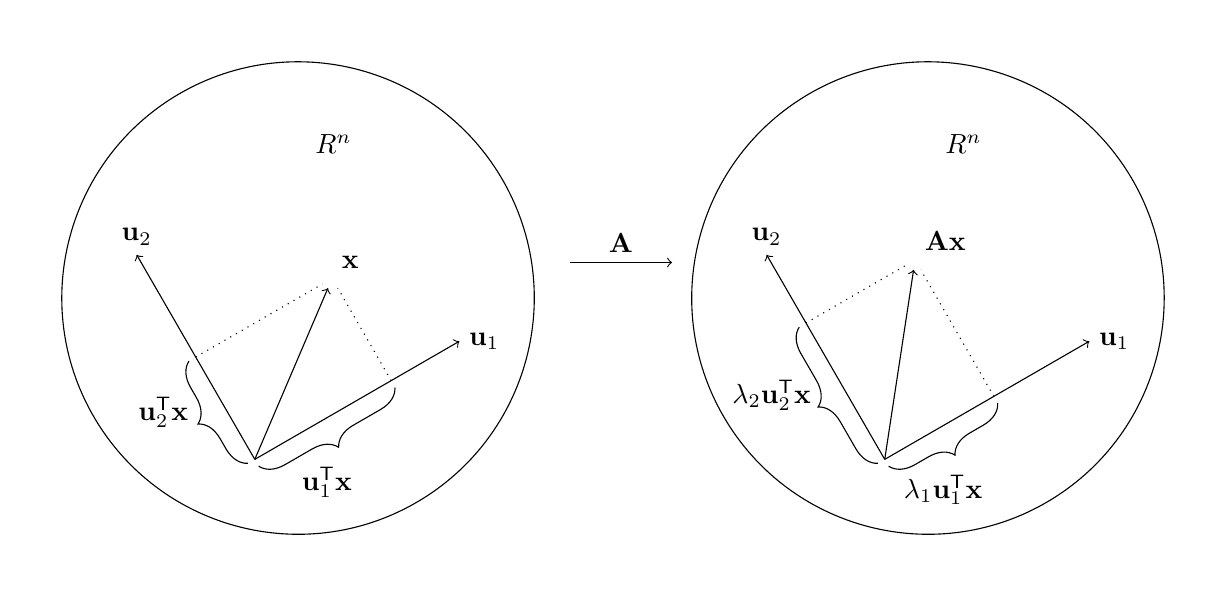
\begin{tikzpicture}
\begin{scope}[rotate = 30]
\node (x) at (2,1.5) {};
  \draw  (1.5,1.5) circle (3cm);
  \draw [->] (0,0) -- (3,0) node[right] {$\mathbf u_1$};
  \draw [->] (0,0) -- (0,3) node[above] {$\mathbf u_2$};
\draw [->] (0,0) -- (x) node[above right] {$\mathbf {x}$};
\draw [dotted] (2,0) -- (x);
\draw [dotted] (0,1.5) -- (x);
\draw [decorate,decoration={brace,amplitude=3mm,mirror},yshift=-1mm] (0,0) -- (2,0) node [midway,yshift=-7mm] { $\mathbf u_1^{\mathsf T} \mathbf x$};
\draw [decorate,decoration={brace,amplitude=3mm},xshift=-1mm] (0,0) -- (0,1.5) node [midway,xshift=-7mm] { $\mathbf u_2^{\mathsf T} \mathbf x$};
\end{scope}
\node at (1,4) {$\mathbb R^n$};

\draw [->] (4,2.5) --  (5.3,2.5)  node [midway,above] {$\mathbf A$};

\begin{scope}[xshift = 8cm]
\begin{scope}[rotate = 30]
\node (x) at (1.6,2) {};
  \draw  (1.5,1.5) circle (3cm);
  \draw [->] (0,0) -- (3,0) node[right] {$\mathbf u_1$};
  \draw [->] (0,0) -- (0,3) node[above] {$\mathbf u_2$};
\draw [->] (0,0) -- (x) node[above right] {$\mathbf {Ax}$};
\draw [dotted] (1.6,0) -- (x);
\draw [dotted] (0,2) -- (x);
\draw [decorate,decoration={brace,amplitude=3mm,mirror},yshift=-1mm] (0,0) -- (1.6,0) node [midway,yshift=-7mm] { $\lambda_1\mathbf u_1^{\mathsf T} \mathbf x$};
\draw [decorate,decoration={brace,amplitude=3mm},xshift=-1mm] (0,0) -- (0,2) node [midway,xshift=-8.5mm] { $\lambda_2\mathbf u_2^{\mathsf T} \mathbf x$};
\end{scope}
\node at (1,4) {$\mathbb R^n$};
\end{scope}
\end{tikzpicture}

\caption{Effect of a real symmetric matrix $\bf A$ of size $n$ on a vector $\bf x$. Only two of the orthogonal eigenvectors are shown. } 
\label{fig:decomp}
\end{figure}

Note that this is a special case of {\em diagonalisation}.  A matrix $\bf A$ is diagonalisable if $\mathbf A = \mathbf {PDP}^{-1}$ (or, equivalently, $\mathbf P^{-1}\mathbf{AP} = \mathbf D$) for some diagonal matrix $\bf D$ and some matrix $\bf P$.  In the case discussed above, where $\bf A$ is real and symmetric, $\bf A$ is diagonalisable with  $\mathbf P = \bf U$ and $\mathbf U^{-1} = \mathbf U^{\mathrm T}$.

%%}%end not in exam

\section{Singular Value Decomposition (SVD)}

Singular Value Decomposition is a method of factorising any ordinary rectangular $m\times n$ matrix.  It is most frequently applied to problems where  $m\ge n$ (more equations than unknowns).

It has  applications in signal processing, pattern recognition, and statistics where it is used for 
 least squares data fitting, regularised inverse problems, finding pseudoinverses and performing principal component analysis (PCA).  The application areas are many and varied but include computational tomography, seismology, weather forecast, image compression, image denoising, genetic analyses and more.
 
It is particularly useful when a given set  of linear equations is singular or very close to 
singular in which case conventional solutions (e.g. by LU decomposition) are either not available or produce senseless results (due to the problems being ill-posed).  In these cases, SVD can diagnose and, in some cases, solve the problem giving an useful numerical answer (though not necessarily the  expected one!).

\subsection{Overview of an SVD}

{\bf SVD} represents an ordinary $m \times n$ matrix $\mathbf{A}$ as 
$\mathbf{A} = \mathbf{UDV}^\mathsf{T}$ where:
\begin{itemize}
\item[$\mathbf{U}$] : an $m \times m$ column-orthogonal matrix; its $m$ columns are the $m$ eigenvectors $\mathbf{u}$ of 
the $m\times m$ matrix $\mathbf{AA}^\mathsf{T}$. The vectors $\{ \mathbf u \}$ are known as the {\em left singular vectors} of $\bf A$.
\item[$\mathbf{V}$] : an $n \times n$ orthogonal matrix; its $n$ columns are the eigenvectors $\mathbf{v}$ of 
the $n\times n$ matrix $\mathbf{A}^\mathsf{T}\mathbf{A}$ . The vectors $\{ \mathbf v \}$ are known as the {\em right singular vectors} of $\bf A$.

\item[$\mathbf{D}$]  : an $m \times n$ matrix whose only non-zero elements are the first $r$ entries on the diagonal where $r$ is the rank of $\bf A$ and  $d_{kk} = \sigma_k = \sqrt \lambda_k$ where $\lambda_k$ is the eigenvalue associated with $\mathbf v_k$.
\end{itemize}
The {\em singular values}, $\sigma_k$ are ordered so that $\sigma_1\ge\sigma_2\ge\ldots\ge\sigma_r > 0$.

Since $\mathbf{A} = \mathbf{UDV}^\mathsf{T}$, we can write
\begin{eqnarray}
\label{eqn:svd} \mathbf{A} & = &\sum_{k = 1}^r \sigma_k \mathbf u_k \mathbf v_k^T \\
\nonumber & = &\sigma_1\mathbf{u}_1\mathbf{v}_1^\mathsf{T}+ 
\sigma_2\mathbf{u}_2\mathbf{v}_2^\mathsf{T }+ \ldots + \sigma_r\mathbf{u}_r\mathbf{v}_r^\mathsf{T}.
\end{eqnarray}
This representation suggests the approximation of $\bf A$ by the truncated series, 
\[
 \mathbf{\widehat A_{\rho}}  = \sum_{k = 1}^{\rho} \sigma_k \mathbf u_k \mathbf v_k^T \mbox{ for } \rho < r.
\]

Notice that when $m > n$ (that is, the problem is over-determined), there are at most $n$ non-zero singular values.  In this case, we can truncate the matrix  $\bf U$ to be $m\times n$ and the matrix $\mathbf D$ to be a $n \times n$ diagonal matrix.  This leaves the sum in Equation \ref{eqn:svd} unaltered as the rows or columns that are removed contribute nothing to that sum. In the following example, we employ this strategy.

{\bf Example}: Find the SVD of the matrix $\bf A$ where 
\[ \mathbf{A}=\left[\begin{array}{rr}0&1\\1&1\\1&0\end{array}\right]
\]
{\bf Solution}:  First find the eigenvectors and eigenvalues of $\mathbf{A}\mathbf{A}^\mathsf{T}$ and $\mathbf{A}^\mathsf{T}\mathbf{A}$.  Since $\bf A$ is $3 \times 2$, we need only find the top two eigenvalues and eigenvectors of each of these matrices.  

\[ \mathbf{A}^\mathsf{T}\mathbf{A}=\left[\begin{array}{rrr}0&1&1\\1&1&0\end{array}\right]
\left[\begin{array}{rr}0&1\\1&1\\1&0\end{array}\right] = \left[\begin{array}{rr}2&1\\1&2\end{array}\right] 
\]
which  has eigenvalues $\lambda_1 = 3$ and $\lambda_2 = 1$.  The associated eigenvectors are, respectively, 
\[ \mathbf{v}_1=\frac{1}{\sqrt{2}}\left[\begin{array}{r}1\\ 1\end{array}\right] \mbox{ and } \mathbf{v}_2=\frac{1}{\sqrt{2}}\left[\begin{array}{r}-1\\ 1\end{array}\right].
\]
Notice that the eigenvectors have been normalised.

Similarly, 
\[ 
\mathbf{A}\mathbf{A}^\mathsf{T}=\left[\begin{array}{rr}0&1\\1&1\\1&0\end{array}\right]
\left[\begin{array}{rrr}0&1&1\\1&1&0\end{array}\right]
=\left[\begin{array}{rrr}1&1&0\\1&2&1\\ 0&1&1\end{array}\right]
\]
The top two eigenvalues are $\mu_1 = 3$ and $\mu_2  = 1$.  Notice that these are the same as the top two eigenvalues of $\mathbf{A}^\mathsf{T}\mathbf{A}$.  The associated eigenvectors are 
\[ \mathbf{u}_1=\frac{1}{\sqrt{6}}\left[\begin{array}{r}1\\ 2\\ 1\end{array}\right] \mbox{ and } 
\mathbf{u}_2=\frac{1}{\sqrt{2}}\left[\begin{array}{r}1\\ 0\\ -1\end{array}\right].
\]
The singular values are given by $\sigma_i = \sqrt \lambda_i$, so $\sigma_1 = \sqrt 3$ and $\sigma_2 = 1$.

We can thus write $\bf A$ as 
\[
\begin{array}{l}
\mathbf{A} = \left[\begin{array}{rr}0&1\\1&1\\1&0\end{array}\right] =
\underbrace{\left[\mathbf{u}_1\;\mathbf{u}_2\right]}_{\mathbf{U}}
\underbrace{\mathrm{diag}(\sigma_1,\sigma_2)}_{\mathbf{D}}
\underbrace{\left[\begin{array}{c}\mathbf{v}_1^\mathsf{T}\\\mathbf{v}_2^\mathsf{T}\end{array}\right]}_{\mathbf{V}^\mathsf{T}}\\
\hspace*{4mm}= 
\underbrace{\left[\begin{array}{rr}1/\sqrt{6}& 1/\sqrt{2}\\
                                                           2/\sqrt{6} & 0                          \\
                                                           1/\sqrt{6} & -1/\sqrt{2}\end{array}\right]}_{\mathbf{U}}
\underbrace{\left[\begin{array}{rr}\sqrt{3}& 0 \\
                                                            0 & 1 \end{array}\right]}_{\mathbf{D}}
\underbrace{\left[\begin{array}{rr}1/\sqrt{2} & 1/\sqrt{2}\\ -1/\sqrt{2} & 1/\sqrt{2}\end{array}\right].}_{\mathbf{V}^\mathsf{T}}
\end{array}
\]
The matrix approximation $\widehat {\mathbf A}_1$ is calculated as follows:
\[
\begin{array}{lll}
\widehat{\mathbf{A}}_1 & = & \sigma_1\mathbf{u}_1 \mathbf{v}_1^\mathsf{T}  \\
& = & 
\sqrt{3} \cdot \frac{1}{\sqrt{6}}\left[ \begin{array}{r} 1 \\ 2\\ 1 \end{array} \right]\cdot\frac{1}{\sqrt{2}}
\left[1\;\;1\right] = \frac{1}{2}
\left[\begin{array}{r} 1\\ 2\\ 1\end{array}\right] \left[1\;\;1\right] = \left[\begin{array}{ll}0.5 & 0.5\\ 1 & 1 \\ 0.5 & 0.5\end{array}\right]\\\\
\end{array}
\]
while the approximation can be extended to  $\widehat {\mathbf A}_2 (= \mathbf A)$ by
\[
\begin{array}{lll}
\widehat{\mathbf{A}}_2 & = & \widehat{\mathbf{A}}_1 + \sigma_2\mathbf{u}_2\mathbf{v}_2^\mathsf{T}\\\\
& \equiv & \left[ \begin{array}{ll}0.5 & 0.5\\ 1 & 1 \\ 0.5 & 0.5\end{array} \right] + 
1\cdot\frac{1}{\sqrt{2}}\left[ \begin{array}{r}1\\ 0\\ -1 \end{array}\right]  \frac{1}{\sqrt{2}}\left[ -1\;\;1 \right] \\ \\
&\equiv & \left[ \begin{array}{ll}0.5 & 0.5\\ 1 & 1 \\ 0.5 & 0.5\end{array} \right] + 
\left[ \begin{array}{rr}-0.5 & 0.5\\ 0 & 0 \\ 0.5 & -0.5\end{array} \right]  = 
\underbrace{ \left[ \begin{array}{rr}0 & 1\\ 1 & 1 \\ 1 & 0\end{array} \right].  }_{\mathbf{A}}
\end{array}
\]

%%\notinexam{
\subsection{How does this all work?\footnote{This section is taken, and condensed, from notes  written by Sze Tan for Physics 707: Inverse Problems.   }} \label{sec:svdexplain}

Recall $\bf A$ is $m\times n$ so that $\mathbf A^T \mathbf A$ is $n\times n$ and $\mathbf {AA}^T$ is $m \times m$.  Both of these product  matrices are square and symmetric.

So, by the result we saw earlier,  $\mathbf A^T\mathbf A$ has $n$ real eigenvalues and a set of $n$ orthonormal eigenvectors (similarly for $\mathbf {AA}^T$ which has $m$ of them).

Let $\mathbf v_i$ be the eigenvectors of $\mathbf {AA}^T$ and $\lambda_i$ be the corresponding eigenvectors and order them so that $\lambda_1 \geq \lambda_2 \geq \ldots \geq \lambda_n \geq 0$. (It can be shown that all eigenvales here are $\geq 0$.)

Similarly, let $\mathbf u_i$ be the eigenvectors of $\mathbf A^T\mathbf A$ and $\mu_i$ be the corresponding eigenvectors and order them so that $\mu_1 \geq \mu_2 \geq \ldots \geq \mu_m \geq 0$.

It turns out that the non-zero eigenvalues of $\mathbf{AA}^T$ are exactly the same as the non-zero eigenvalues of $\mathbf A^T\mathbf A$.  Suppose there are $r$ such non-zero eigenvalues, so that $\lambda_{r+1} = \ldots = \lambda_n = 0$ and $\mu_{r+1} = \ldots = \mu_m = 0$.

$r$ is called the {\em rank} of $\bf A$ (and of $\mathbf A^T$). Clearly, $r \leq m$ and $r \leq n$.

Now, for $k = 1,\ldots, r$, it can be shown that we have 
\[
\mathbf {Av}_k = \sigma_k \mathbf u_k \mbox{ and } \mathbf A^T \mathbf u_k = \sigma_k \mathbf v_k
\]
where $\sigma_k = \sqrt \lambda_k = \sqrt \mu_k$.  And, also that, for $k > r$,
\[
\mathbf {Av}_k = 0 \mbox{ and } \mathbf A^T \mathbf u_k =0.
\]
The equations $\mathbf {Av}_k = \sigma_k \mathbf u_k$ for  $k \leq r$ together with $\mathbf {Av}_k = 0$ for $k >r$ tell us how $\bf A$ acts on the orthonormal set of vectors $\{ \mathbf v_k \}$.  Since this set is  a basis for $\mathbb R^n$, the equations give a complete description of the action of $\bf A$, so that we can write 
\begin{equation} \mathbf A = \sum_{k = 1}^r \sigma_k \mathbf u_k \mathbf v_k ^{\mathrm T}. \label{eqn:svd2}
\end{equation}
A similar argument shows that 
\[ \mathbf A ^{\mathrm T}= \sum_{k = 1}^r \sigma_k \mathbf v_k \mathbf u_k ^{\mathrm T}. \]

The orthonormal vectors $\{ \mathbf v_k \}$ are known as the {\em right singular vectors}, the vectors $\{ \mathbf u_k \}$ are known as the {\em left singular vectors}, and the scalars $\{ \sigma_k \}$ are called the {\em singular values} of the matrix $\mathbf A$.

The singular value decomposition allows us to understand the action of $\mathbf A$ on a vector $\mathbf x$ as 
\[ \mathbf {Ax} = \sum_{k = 1}^r \mathbf u_k \sigma_k ( \mathbf v_k ^{\mathrm T} \mathbf x). 
\]
 which can be interpreted as having  three stages:
\begin{enumerate}
\item It resolves the input vector along each of the right singular vectors $\mathbf v_k$, the component of the input
vector along the $k$th singular vector being given by $\mathbf v_k^T \mathbf x$,
\item The amount along the $k$th direction is multiplied by the singular value $\sigma_k$,
\item The product tells us how much of the $k$th left singular vector $\mathbf u_k$ is present in the product $\mathbf {Ax}$.
\end{enumerate}
This is illustrated in Figure \ref{fig:decomp2}.


\begin{figure}[hbtp]
\centering
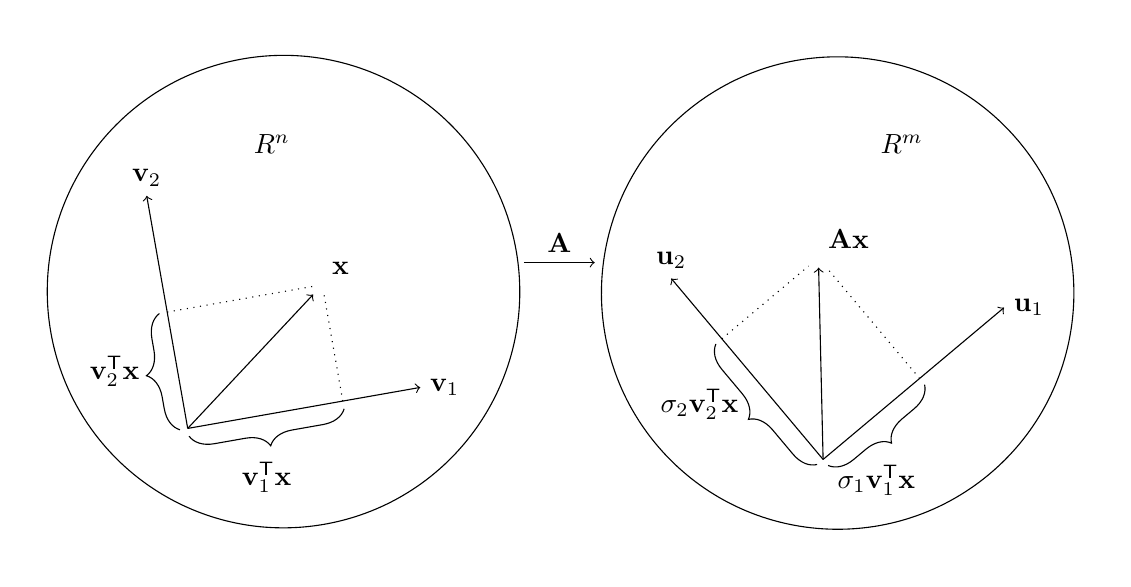
\begin{tikzpicture}
\begin{scope}[rotate = 10,yshift = 4mm]
\node (x) at (2,1.5) {};
  \draw  (1.5,1.5) circle (3cm);
  \draw [->] (0,0) -- (3,0) node[right] {$\mathbf v_1$};
  \draw [->] (0,0) -- (0,3) node[above] {$\mathbf v_2$};
\draw [->] (0,0) -- (x) node[above right] {$\mathbf {x}$};
\draw [dotted] (2,0) -- (x);
\draw [dotted] (0,1.5) -- (x);
\draw [decorate,decoration={brace,amplitude=3mm,mirror},yshift=-1mm] (0,0) -- (2,0) node [midway,yshift=-7mm] { $\mathbf v_1^{\mathsf T} \mathbf x$};
\draw [decorate,decoration={brace,amplitude=3mm},xshift=-1mm] (0,0) -- (0,1.5) node [midway,xshift=-7mm] { $\mathbf v_2^{\mathsf T} \mathbf x$};
\end{scope}
\node at (1,4) {$\mathbb R^n$};

\draw [->] (4.2,2.5) --  (5.1,2.5)  node [midway,above] {$\mathbf A$};

\begin{scope}[xshift = 8cm]
\begin{scope}[rotate = 40]
\node (x) at (1.6,2) {};
  \draw  (1.5,1.5) circle (3cm);
  \draw [->] (0,0) -- (3,0) node[right] {$\mathbf u_1$};
  \draw [->] (0,0) -- (0,3) node[above] {$\mathbf u_2$};
\draw [->] (0,0) -- (x) node[above right] {$\mathbf {Ax}$};
\draw [dotted] (1.6,0) -- (x);
\draw [dotted] (0,2) -- (x);
\draw [decorate,decoration={brace,amplitude=3mm,mirror},yshift=-1mm] (0,0) -- (1.6,0) node [midway,yshift=-7mm] { $\sigma_1\mathbf v_1^{\mathsf T} \mathbf x$};
\draw [decorate,decoration={brace,amplitude=3mm},xshift=-1mm] (0,0) -- (0,2) node [midway,xshift=-8.5mm] { $\sigma_2\mathbf v_2^{\mathsf T} \mathbf x$};
\end{scope}
\node at (1,4) {$\mathbb R^m$};
\end{scope}
\end{tikzpicture}
%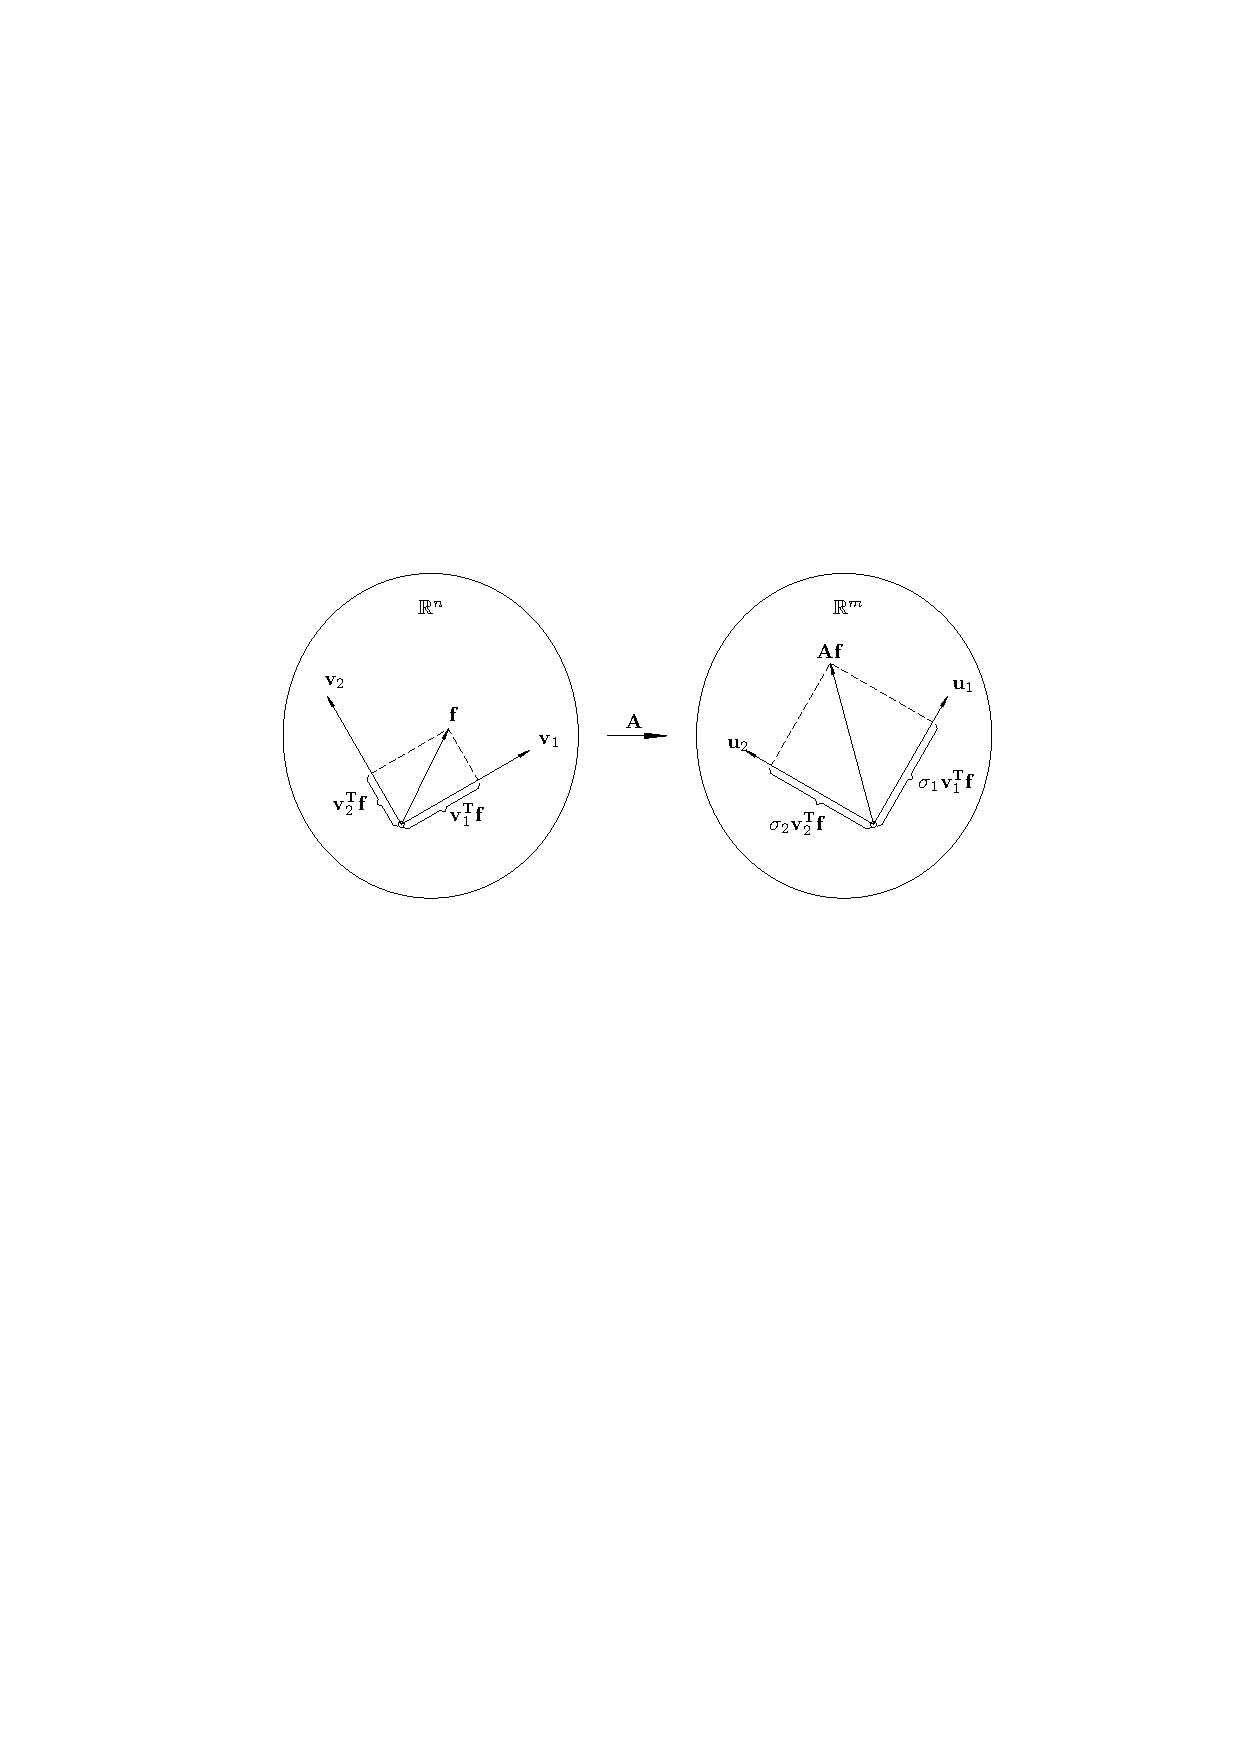
\includegraphics[width=12cm]{figures/MatrixDecomp2.pdf}
\caption{Effect of a rectangular  matrix $\bf A$ of size $m\times n$ on a vector $\bf x$. Only two of the orthogonal eigenvectors are shown. }
\label{fig:decomp2}
\end{figure}
%%} %end not in exam


\subsection{Structure of SVD}

In the overdetermined case, in which $m > n$, so that we have more equations than unknowns,  we have the following structure:

\tikz[scale=1.5]{ \small 
\fill[pink] (0,-0.5) -- (0,0.25) -- (0.5,0.25) -- (0.5,-0.5); 
\draw[blue] (0,-0.5) -- (0,0.25) -- (0.5,0.25) -- (0.5,-0.5) -- cycle; 
\node at (0.25,0) {$\mathbf{A}$};
\node at (0.7,0) {$=$};
\fill[pink] (0.9,-0.5) -- (0.9,0.25) -- (1.4,0.25) -- (1.4,-0.5); 
\draw[blue] (0.9,-0.5) -- (0.9,0.25) -- (1.4,0.25) -- (1.4,-0.5) -- cycle; 
\node at (1.15,0) {$\mathbf{U}$};
\fill[pink] (1.5,-0.25) -- (1.5,0.25) -- (2,0.25) -- (2,-0.25); 
\draw[blue] (1.5,-0.25) -- (1.5,0.25) -- (2,0.25) -- (2,-0.25) -- cycle; 
\node at (1.75,0) {$\mathbf{D}$};
\fill[pink] (2.1,-0.25) -- (2.1,0.25) -- (2.6,0.25) -- (2.6,-0.25); 
\draw[blue] (2.1,-0.25) -- (2.1,0.25) -- (2.6,0.25) -- (2.6,-0.25) -- cycle; 
\node at (2.35,0) {$\mathbf{V}^{\mathsf{T}}$};
}

In the underdetermined case, in which $m < n$, so that we have fewer equations than unknowns,  we have the following structure:

\tikz[scale=1.5]{ \small 
\fill[pink] (0,0) -- (0,0.25) -- (0.5,0.25) -- (0.5,0); 
\draw[blue] (0,0) -- (0,0.25) -- (0.5,0.25) -- (0.5,0) -- cycle; 
\node at (0.25,0.12) {$\mathbf{A}$};
\node at (0.7,0.12) {$=$};
\fill[pink] (0.9,0) -- (0.9,0.25) -- (1.4,0.25) -- (1.4,0); 
\draw[blue] (0.9,0) -- (0.9,0.25) -- (1.4,0.25) -- (1.4,0) -- cycle; 
\node at (1.15,0.12) {$\mathbf{U}$};
\fill[pink] (1.5,-0.25) -- (1.5,0.25) -- (2,0.25) -- (2,-0.25); 
\draw[blue] (1.5,-0.25) -- (1.5,0.25) -- (2,0.25) -- (2,-0.25) -- cycle; 
\node at (1.75,0.12) {$\mathbf{D}$};
\fill[pink] (2.1,-0.25) -- (2.1,0.25) -- (2.6,0.25) -- (2.6,-0.25); 
\draw[blue] (2.1,-0.25) -- (2.1,0.25) -- (2.6,0.25) -- (2.6,-0.25) -- cycle; 
\node at (2.35,0.12) {$\mathbf{V}^{\mathsf{T}}$};
}


Note that, in the overdetermined  case,  we truncate $\mathbf U$ and $\mathbf D$ since there are at most $r \leq n < m$ non-zero singular values of $\mathbf A$ we can omit the $\mathbf u_i$ that contribute nothing to matrix product.


The matrix $\mathbf V$ is orthonormal, so $\mathbf {VV}^T = \mathbf V^T\mathbf V = \mathbf I_n$.  $\mathbf U$ is orthonormal when $m \geq n$, but if $m < n$, the singular values $\sigma_j = 0$ for $j = m+1,\ldots, n$ and the corresponding columns of $\mathbf U$ are also 0 so that $\mathbf{UU}^T = \mathrm{diag}(1,\ldots,1,0,\ldots,0)$ where only the first $m$ elements of the diagonal are 1 and the elements from $m+1$ to $n$ are zero.

Note that the SVD of matrix $\mathbf A$ is only unique up to permutations of the columns/rows.  For this reason, we insist that the singular values and corresponding singular vectors are arranged so that the singular values are in descending order $\sigma_1 \geq \sigma_2 \geq \ldots$.  Even then, some of the $\sigma_i$'s may have the same value so columns of $\mathbf U$ and $\mathbf V$ could be permuted.  Aside from these possible permuations, the representation is unique.  Be aware when calculating the SVD with various software that the you may need to enforce this canonical representation.


\subsection{Condition number of a matrix}

The concept of a condition number was introduced in  Section \ref{sec:why}.  This concept can be applied to a matrices and is useful, for example, when considering solutions to the equation $\mathbf {Ax} = \mathbf b$.  Solutions to this equation will change greatly with  small changes in $\mathbf b$ when $\mathbf A$ has a large condition number, while the small changes in  $\mathbf b$ will lead to only small changes in the solution when the matrix has a small condition number.  We can define the condition number of a matrix as the maximum of the  ratio of the relative error in $\mathbf x$ divided by the relative error in $\mathbf b$, where the maximum is taken over all possible $\mathbf x$ and $\mathbf b$.

To give a full description of how to derive the condition number of $\mathbf A$, we would have to introduce matrix norms which we do not have time to do here.  Instead, we simply present the result here that the condition number of $\mathbf A$ can be defined as the ratio of the largest to the smallest non-zero singular values:
\[ cond(\mathbf A) = \frac{\sigma_{\max}}{\sigma_{\min}}. \]
If the smallest singular value of $\mathbf A$ is 0,  $\mathbf A$ is singular (has no inverse) but the condition number of $\mathbf A$ is still defined.



The condition number of $\mathbf A$ is considered to be large, and the matrix is {\em ill-conditioned},  if roughly $\log(cond(\mathbf A)) \geq k $ where $k$ is the number of digits of precision in the matrix entries.

{\bf Example}: Find the condition number of the matrix $\mathbf A = \left[\begin{array}{ll}2 & -3\\1&-1\end{array}\right]$

{\bf Solution}: Using a matrix algebra package, find the singular values of $\mathbf A$ to be $3.864$ and $ 0.259$, so $cond(\mathbf A) = \frac {3.864}{0.259} \approx 14.9$.  \sqend

{\bf Example}: The singular values of the matrix  $\mathbf A = \left[\begin{array}{ll} 1.2969 & 0.8648 \\ 0.2161 & 0.1441 \end{array}\right]$ are approximately $1.58$ and $6.33\times 10^{-9}$ so the condition number is about $2.5\times 10^8$.  This very large condition number means that $\mathbf A$ is an  ill-conditioned matrix.

Ill-conditioning  means that standard approaches to solving linear  systems can be very unstable.  For example, consider the  linear system $\mathbf{Ax} = \mathbf b$ where $\mathbf b = \left[\begin{array}{r} 0.8642 \\ 0.1140 \end{array}\right]$.  This has the exact solution $\mathbf x = \left[\begin{array}{r} 2 \\ -2 \end{array}\right]$. 

But standard matrix software ({\tt linsolve} in Matlab), gives the solution as $\left[\begin{array}{r} 2.59  \\ -3.89  \end{array}\right]\times 10^6$ which is radically wrong!

It also means that if some number in the system is measured slightly differently, the results we get can change enormously.  For example, if  the measurement vector $\mathbf b$ is just slightly different, say $\mathbf b = \left[\begin{array}{r} 0.86419999 \\ 0.11400001 \end{array}\right]$, then the exact solution is now close to $\mathbf x = \left[\begin{array}{r} 0.9911 \\ -0.4870 \end{array}\right]$ which represents an enormous change in the solution relative to the small change in the original system. \sqend

%%\notinexam{




%\subsection{Applications of SVD}

We'll see in a later section on pseudo-inverses how the SVD can be used to solve the linear system $\mathbf{Ax} = \mathbf b$.


\subsubsection{Image compression}

See slides and assignment 1.

\subsubsection{Gene expression}

Abstract from Alter et al, 2000, {\em Singular value decomposition for genome-wide expression data processing and modeling},  \url{http://www.pnas.org/content/97/18/10101.full}: We describe the use of singular value decomposition in transforming genome-wide expression data from genes $\times$ arrays space to reduced diagonalized ``eigengenes'' $\times$ `eigenarrays'' space, where the eigengenes (or eigenarrays) are unique orthonormal superpositions of the genes (or arrays). Normalizing the data by filtering out the eigengenes (and eigenarrays) that are inferred to represent noise or experimental artifacts enables meaningful comparison of the expression of different genes across different arrays in different experiments. Sorting the data according to the eigengenes and eigenarrays gives a global picture of the dynamics of gene expression, in which individual genes and arrays appear to be classified into groups of similar regulation and function, or similar cellular state and biological phenotype, respectively. After normalization and sorting, the significant eigengenes and eigenarrays can be associated with observed genome-wide effects of regulators, or with measured samples, in which these regulators are overactive or underactive, respectively. 

%
%
%
% \newpage
%%}%end not in exam


\subsection{Principal Components Analysis (PCA)}



PCA is a common technique for identifying patterns in high-dimensional data.  It  transforms   the original correlated measurements into uncorrelated measurements.
 One of the main uses of PCA is as a dimension reduction tool, in which only the directions in which the data varies the most are considered.  This can lead to enormous simplifications of the data and provide insights for a wide variety of data.   PCA is alternatively known as  the Karhunen-Lo\'eve transform (KLT), the Hotelling transform or proper orthogonal decomposition (POD)
 
 These new coordinate axes (along which the data varies the most) are are known as {\em principal components} and are, by construction, orthogonal.

 A useful visualisation tool to aid your understanding of PCA is at \href{http://setosa.io/ev/principal-component-analysis/}{http://setosa.io/ev/principal-component-analysis/}.


Suppose we have a  $m \times n$ matrix of measurement data $A$.  For example, $n$ trials where $m$ properties were measured in each trial.  Then, if $\mathbf a_i$ are the measurements from the $i$th trial,  
\[
\mathbf{A} = \left[\begin{array}{cccc}\mathbf{a}_1 & \mathbf{a}_2 & \ldots & \mathbf{a}_n \end{array}\right]
= \left[\begin{array}{cccc}
a_{11} & a_{12} & \ldots & a_{1n}\\
a_{21} & a_{22} & \ldots & a_{2n}\\
\vdots  &  \vdots & \ddots & \vdots \\
a_{m1} & a_{m2} & \ldots & a_{mn}\\
 \end{array}\right].
\]
For example, $\bf A$ could be $n = 100$ observations of the position of an object measured in $m = 3$ dimensions.

%In the following, assume that the columns of $\mathbf A^{\mathsf T}$ have been centred, so that the mean of each column is 0 (the columns of $\mathbf A^T$ are just the rows of $\mathbf A$ so correspond to each dimension of the measurements). If this is not already the case, it can be achieved by subtracting the mean of each column of $\mathbf A^T$ from each element of that column. That is, set element  \[a_{ij} = a_{ij}- \sum_{j = 1}^n a_{ij}/n\] to centre the rows of $\mathbf A$ and, therefore, the columns of $\mathbf A^T$.  This is a critical assumption and allows us to concentrate on the variance. 
In the following, assume that the rows of $\mathbf A$ have been centred, so that the mean of each row is 0 (each rows of $\mathbf A$  corresponds to a dimension in the original data). If this is not already the case, it can be achieved by subtracting the mean of each row of $\mathbf A$ from each element of that row. That is, set element  \[a_{ij} = a_{ij}- \sum_{j = 1}^n a_{ij}/n\] to centre the rows of $\mathbf A$.  This is a critical assumption and allows us to concentrate on the variance. 

Each observation $\bf A$ is just the $m$-vector $\mathbf a_i$. The idea of PCA is to chose a new basis $\mathbf u_1, \ldots, \mathbf u_k$ to express the data points (the $\mathbf a_i$'s) so that the variance of the measurements  is greatest in the direction of $\mathbf u_1$, the next greatest variance is in the direction of $\mathbf u_2$ and so on, down to $\mathbf u_k$.  Ideally, $k < m$.

Define the {\em covariance matrix} of $\mathbf A$ by 
\[\mathbf \Sigma = \frac 1 {n-1} \mathbf {AA}^T. \] %\approx \frac 1 {n} \mathbf {AA^T} .\]
Then $\mathbf \Sigma$ is an $m \times m$ matrix where the diagonal terms of $\mathbf \Sigma $ are the variance of the $i$th dimension of the measurement, while the off-diagonal terms of $\mathbf \Sigma $ are the covariances between different measurements.  

It turns out that the best basis to choose are the $k$ eigenvectors of $\mathbf \Sigma$  corresponding its $k$ largest eigenvalues.  These are known as the {\em principal components} of $\mathbf A$.  Call them $\mathbf u_1, \ldots, \mathbf u_k$ and form the matrix 
\[
\mathbf U_k = [\mathbf u_1, \ldots, \mathbf u_k]
\]
From results we have seen earlier about symmetric matrices, this an orthogonal matrix.  We include the subscript $k$ as we may decide to truncate this matrix by including only the eigenvectors corresponding to the largest eigenvalues.  That is, if $\mathbf \Sigma$ has $K$ eigenvectors and associated eigenvalues, and the largest $k$ eigenvalues are substantially larger than the remaining $K-k$, it is reasonable to form $ \mathbf U_k$ containing only the most significant $k$ eigenvectors.



We can now represent  the original measurements, $\mathbf A$, in this this new co-ordinate system.   The amount of measurement vector $\mathbf a_i$ in direction $\mathbf u_j$ is given by $\mathbf u_j^\top  \mathbf a_i$:  this is the  $j$th coordinate of $\mathbf a_i$ in this new coordinate system.  So if we consider just the two dimension space defined by the top two principal components,  $\mathbf a_i$ has coordinates  \[ \mathbf{U}_2^\mathsf{T} \mathbf a_i  = 
\left[\begin{array}{c}
\mathbf{u}_1^\mathsf{T}\\ \mathbf{u}_2^\mathsf{T} 
\end{array}\right] \mathbf a_i 
= 
\left[\begin{array}{c}
\mathbf{u}_1^\mathsf{T}\mathbf a_i \\ \mathbf{u}_2^\mathsf{T} \mathbf a_i
\end{array}\right]. \]

We usually consider this space independently of how it relates to the original $m$-dimensional space but we can consider it as embedded in the original  space.
%and he original points projected onto that embedded lower dimensional space.  
To find the coordinates of a point in this embedded space, define the projection matrix, $\mathbf P_k$  by
\[
\mathbf{P}_k = \mathbf{U}_k\mathbf{U}_k^\mathsf{T} = 
\left[\begin{array}{cccc}
\mathbf{u}_1 & \mathbf{u}_2 & \ldots & \mathbf{u}_k
\end{array}\right]
\left[\begin{array}{c}
\mathbf{u}_1^\mathsf{T}\\ \mathbf{u}_2^\mathsf{T}\\ \vdots \\ \mathbf{u}_k^\mathsf{T}
\end{array}\right]
\]
so that each measurement vector $\mathbf a_i$ is projected via $\mathbf P_k \mathbf a_i$.  

One interpretation of PCA is that the projection $\mathbf{P}_k$ is chosen to minimise the projection error
$\sum_{j=1}^n\|\mathbf{a}_j-\mathbf{P}_k\mathbf{a}_j\|^2$


{\bf Example:} Find the principal components of the data matrix $\mathbf A$ where 
\[ \mathbf A= \left[ 
\begin{array}{rrrrrr}
  -4   & 3  & -5  & 18 &   6  & -5 \\
    2  &  6  & -2  & 10   & 1 &  -1 \\ 
    7 &  11  &  3 &   6  &  9 &   3 \\
\end{array} \right].
\]
Find the amount of the first principal component in the first measurement vector of $\mathbf A$ (that is, the first column), and calculate the projection matrix for projecting  $\mathbf A$ onto the first two principal components.


{\bf Solution:} First, centre the rows of $\mathbf A$ so that each row has mean zero.  Call this centred matrix $\mathbf B$.
\[ \mathbf B= \left[ 
\begin{array}{rrrrrr}
 -6.1667 & 0.8333 & -7.1667 & 15.8333  & 3.8333 & -7.1667 \\
 -0.6667 & 3.3333 & -4.6667 & 7.3333 & -1.6667 & -3.6667\\
  0.5 & 4.5 & -3.5 & -0.5 & 2.5 & -3.5\\
\end{array} \right].
\]
Now form the covariance matrix for the centred data matrix,  $\mathbf{\Sigma}  = \frac 1 n \mathbf B \mathbf B^{\mathsf T}$:
\[ \mathbf \Sigma = \frac 1 5 \left[ 
\begin{array}{rrr}
 406.8333 &176.3333   &  52.5\\
 176.3333 & 103.3333 &  36.0\\
  52.5000  & 36.0000 & 51.5\\
\end{array} \right].
\]
This matrix has eigenvalues $99.31, \;  9.46$ and  $ 3.561$ corresponding to eigenvectors 
\[ [\mathbf u_1, \mathbf u_2, \mathbf u_3] =  \left[ 
\begin{array}{rrr}
 0.8987 & 0.2829 & 0.3352 \\ 
 0.4158 & -0.3062 & -0.8564 \\ 
 0.1396 & -0.9090 & 0.3928  
 \end{array} \right] = \mathbf U.
\]
These eigenvectors are the principal components of $\mathbf A$ (and of $\mathbf B$).  

The amount  of the first principal component in $\mathbf a_1$ is $$\mathbf u_1^\top \mathbf a_1 =   
[0.8987, 0.4158, 0.1396] \left[\begin{array}{r}
-4 \\ 2\\ 7 \end{array} \right] = -1.756.
$$

To project   $\mathbf A$ into the  coordinate system defined by the first two principal components, form the projection matrix, \[\mathbf P_2  =  \mathbf{U}_2\mathbf{U}_2^\mathsf{T} = \left[ 
\begin{array}{rrr}
 0.8987 & 0.2829  \\
 0.4158 &-0.3062  \\
 0.1396 & -0.9090 \\
\end{array} \right] \left[ 
\begin{array}{rrr}
 0.8987 & 0.4158 &  0.1396 \\ 
 0.2829  & -0.3062 & -0.9090 \\
\end{array} \right]  =
\left[ 
\begin{array}{rrr}
  0.8877 &0.2870 &-0.1316 \\
  0.2870& 0.2666 & 0.3364\\
 -0.1316& 0.3368 & 0.8457\\
\end{array} \right] 
\]


%%\notinexam{
\subsection{Examples}
\label{sec:svdexamples}
See associated slides for population structure in Europe (Novembre et al, Nature 2008, \url{http://www.nature.com/nature/journal/v456/n7218/full/nature07331.html} )and Eigenfaces.

The ``eigenfaces'' example in the slides was developed by Matthew Turk and Alex Pentland (Journal of Cognitive Neuroscience, 1991, v3 (1)). The following quote is from their abstract:
\begin{quote}
We have developed a near-real-time computer system that can locate and track a subject's head, and then recognize the person by comparing characteristics of the face to those of known individuals. ... The system functions by projecting face images onto a feature space that spans the significant variations among known face images. The significant features are known as "eigenfaces," because they are the eigenvectors (principal components) of the set of faces; they do not necessarily correspond to features such as eyes, ears, and noses. The projection operation characterizes an individual face by a weighted sum of the eigenface features, and so to recognize a particular face it is necessary only to compare these weights to those of known individuals. Some particular advantages of our approach are that it provides for the ability to learn and later recognize new faces in an unsupervised manner, and that it is easy to implement using a neural network architecture.
\end{quote}
% 
%%}%end not in exam

\subsection{What is connection between PCA and SVD?}

Given $\mathbf A$  such that the rows of $\mathbf A$ have zero mean, define $\mathbf Y = \frac 1 {\sqrt {n-1}} \mathbf A^T$ (which has  columns with zero mean).  Then $\mathbf Y^T\mathbf Y = \mathbf \Sigma$, the covariance of $\mathbf A$.  We have seen  that the principal components of $\mathbf A$ are the eigenvectors of $\mathbf \Sigma$. 

Now, if we calculate the SVD of $\mathbf Y$ to get $\mathbf Y = \mathbf{UDV}^T$, the columns of $\mathbf V$ are the eigenvectors of $\mathbf Y^T \mathbf Y = \mathbf \Sigma$. Therefore, the columns of $\mathbf V$ are the principal components of $\mathbf A$.
 

\subsection{Problems with SVD and PCA}

As we have seen, SVD and PCA are powerful analysis tools and SVD is a very stable procedure.  They do not, however, come free of cost.  

The time complexity of SVD is $O(m^2n + n^3)$ to calculate all of $\mathbf U, \mathbf V$ and $\mathbf D$ (where, typically, $m \gg n$) while faster algorithms are available when some elements of the SVD are not required.

However, the matrices  $\mathbf{U}$ and $\mathbf{V}$ are not at all {\em sparse}, where we say a matrix is sparse when it mainly consists of zeros. Spareness is a commonly assumed property in large systems as it reflects the observation that most effects are local and do not influence all parameters in the system ---  a large world  with small neighbourhoods.  Sparse matrices are typically computationally efficient to work with and store. 

A second potential set-back is that SVD and PCA only work with data that can be (coherently) expressed as a two dimensional array (that is, a matrix).  When data naturally has 3 or 4 dimensions arrays ({\em tensors}), as is common in many engineering applications, there is no perfect analogue to SVD or PCA or even eigenvectors.  

Finally, when using PCA for data analysis,  you should be aware of the strong assumptions being made.  In particular, dependencies in the data are assumed to be linear, which may not be the case.  PCA and SVD will always give an answer but it is up to the user to interpret whether or not it is a valid answer to any question they are interested in.
   

\section{Least squares} \label{sec:leastsquares}


\begin{figure}[h]
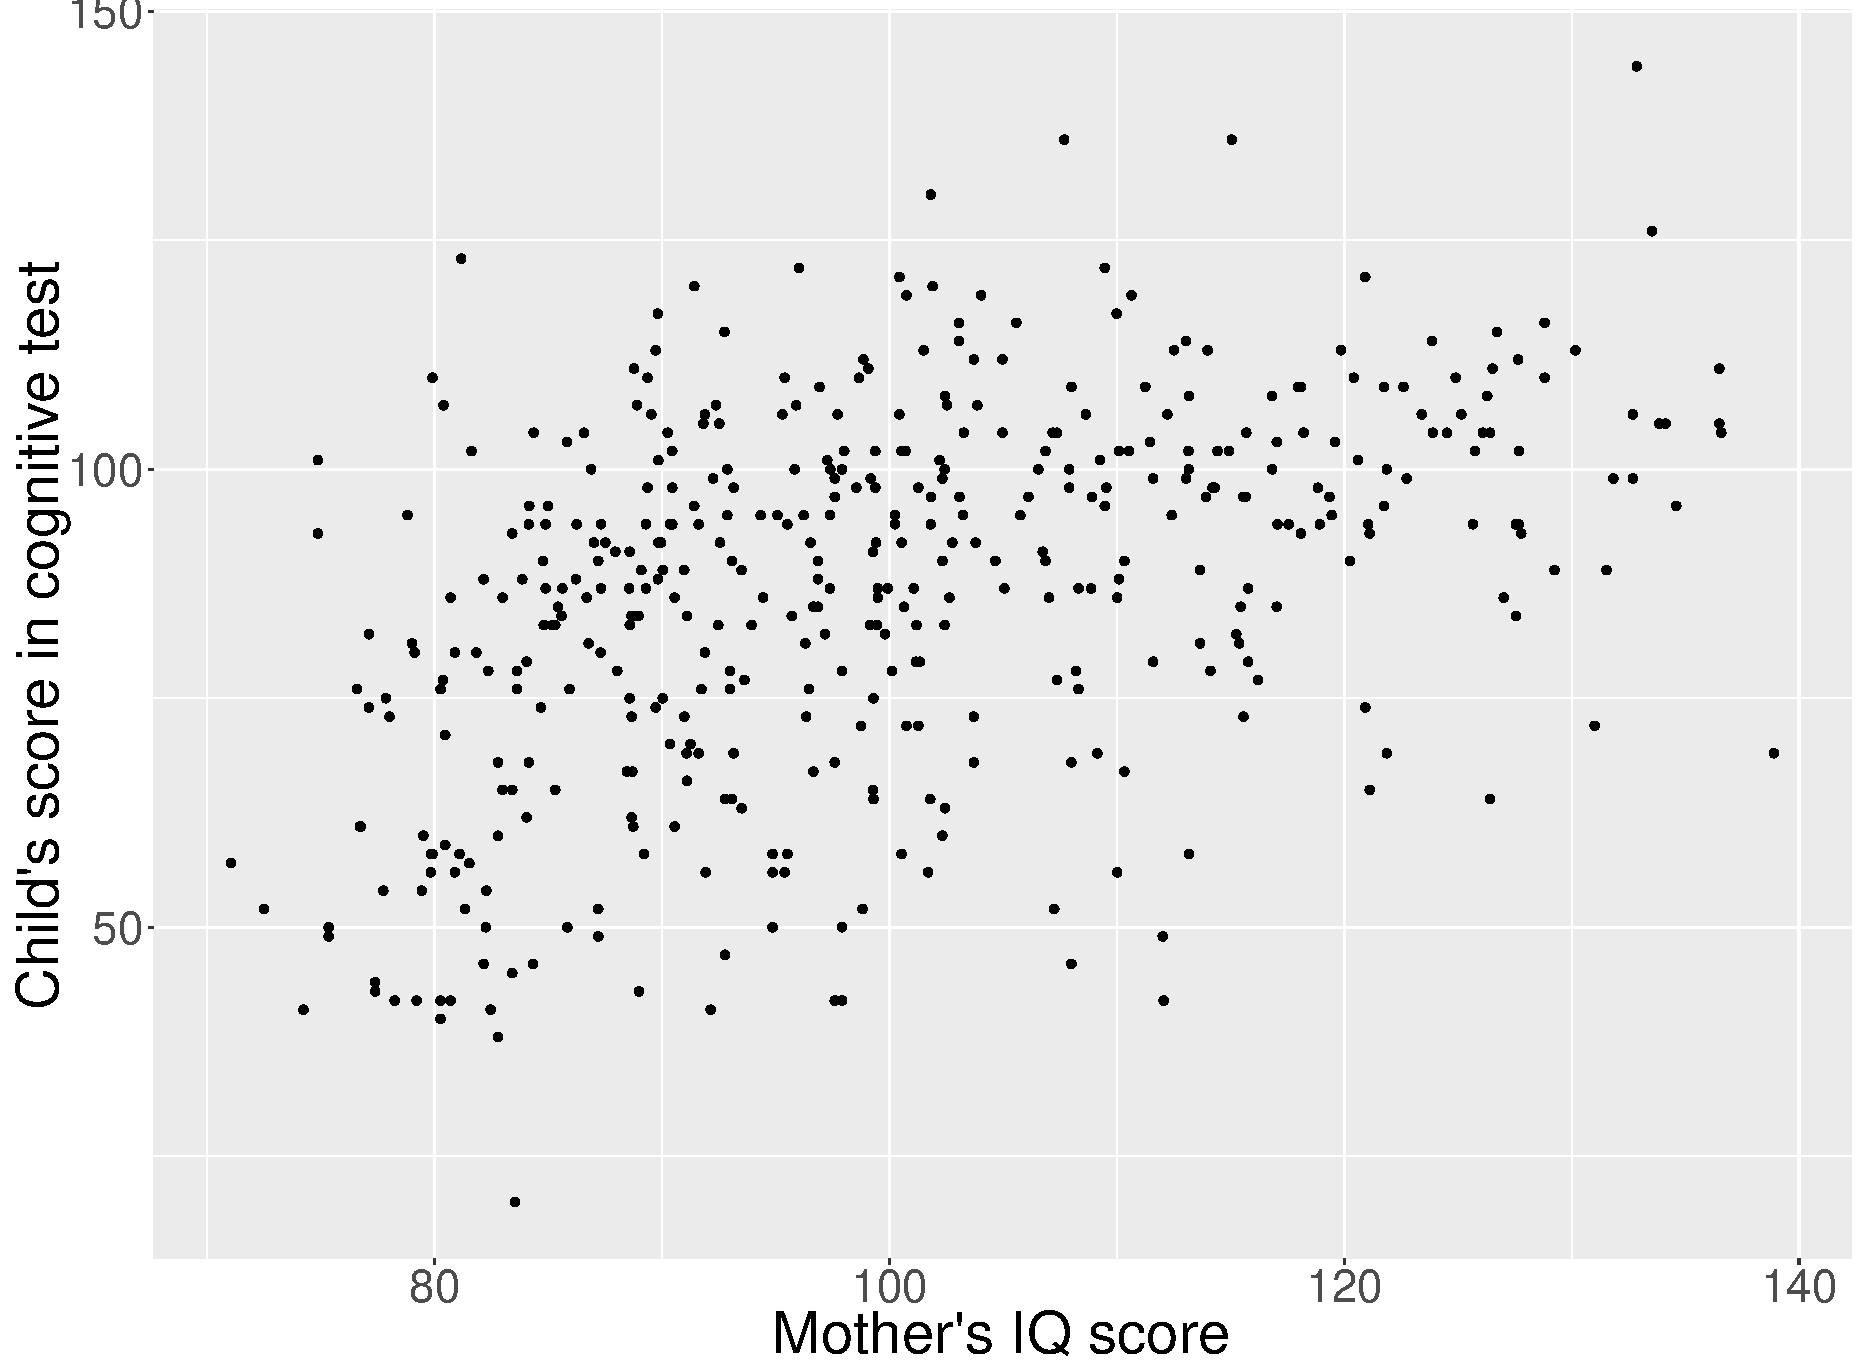
\includegraphics[width=6cm]{figures/kidiq}
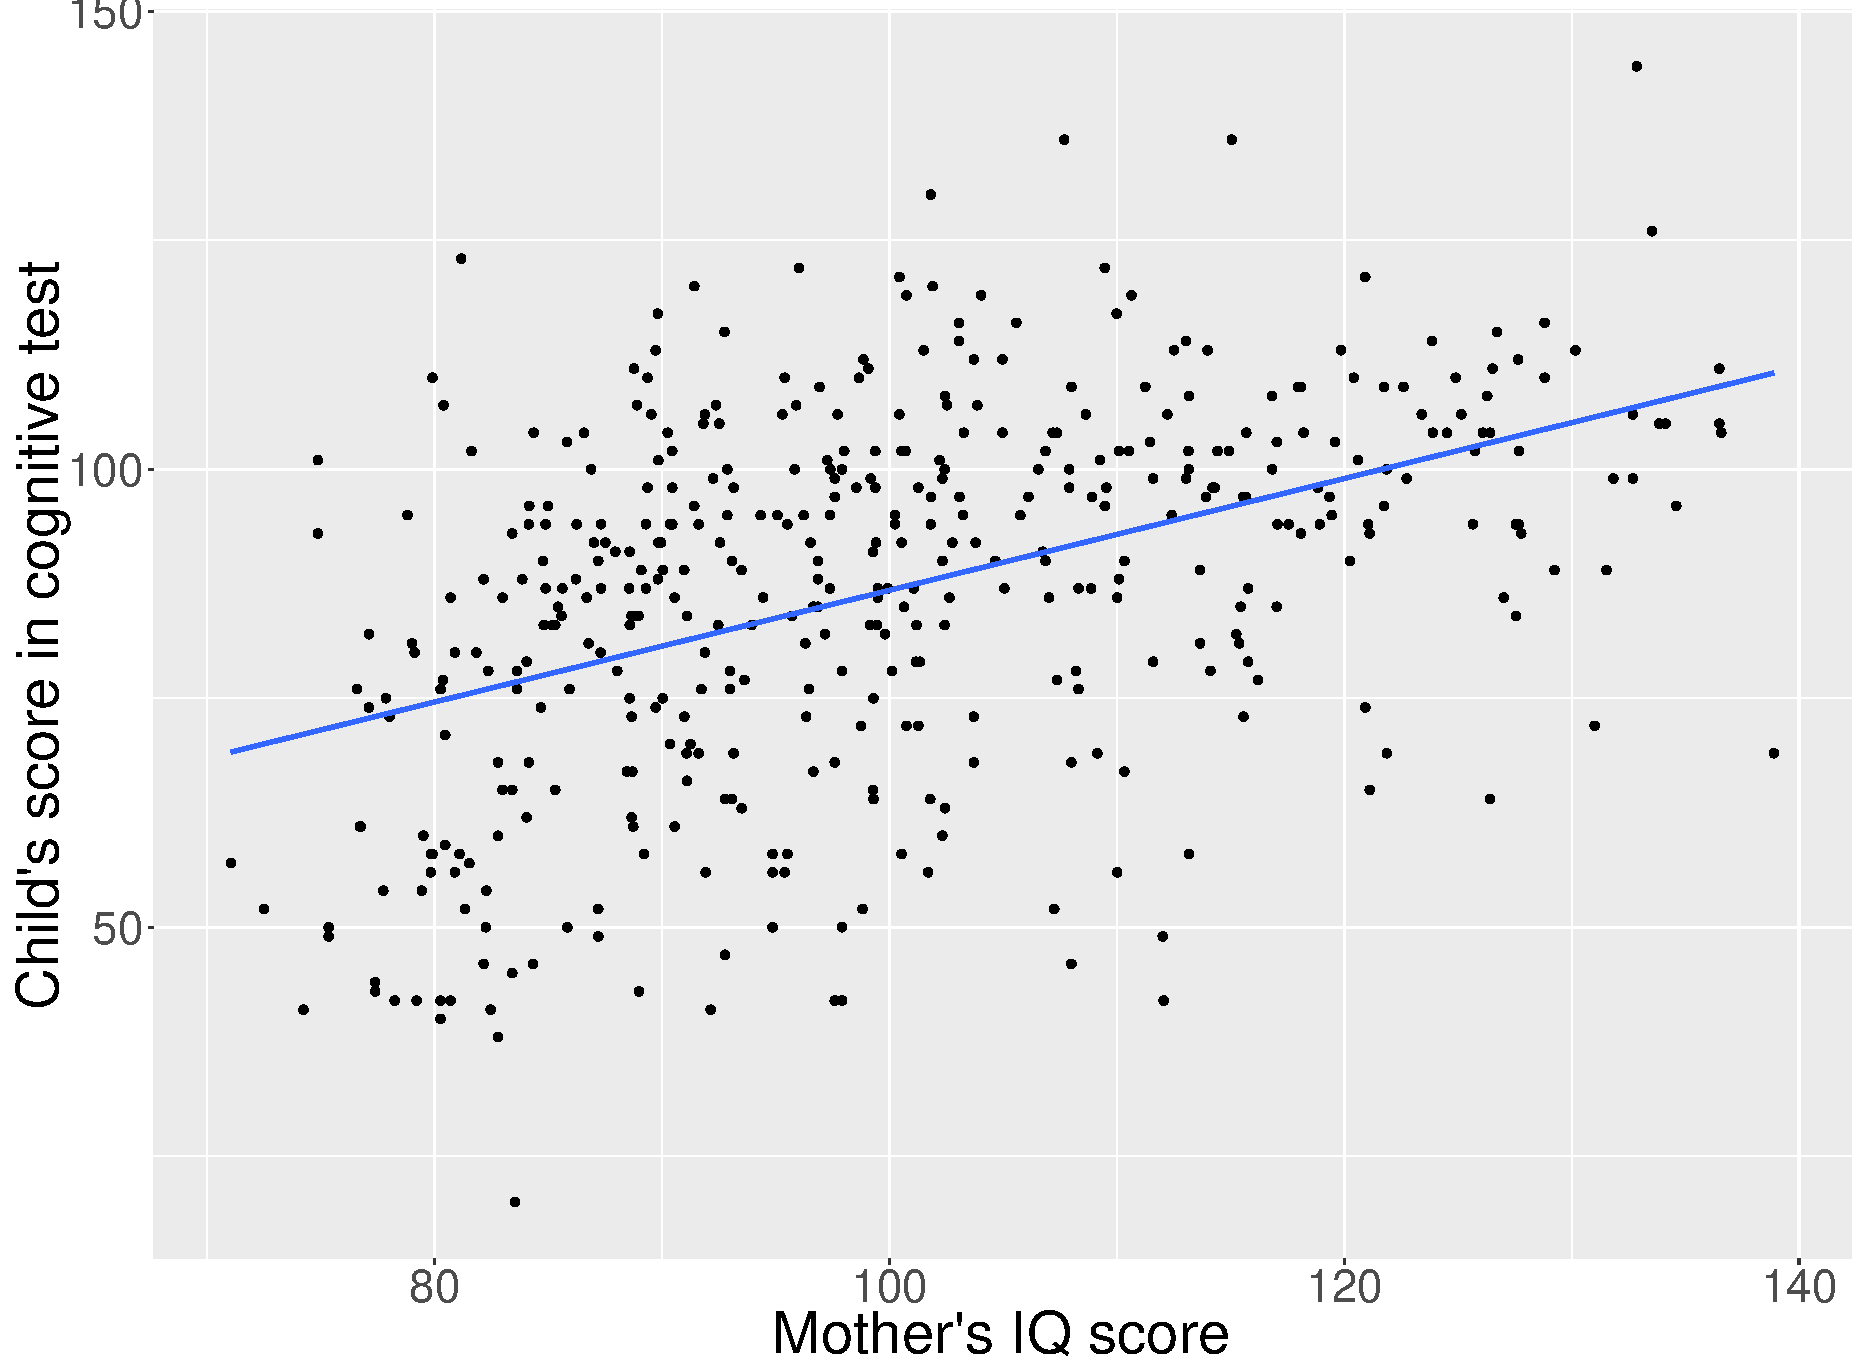
\includegraphics[width=6cm]{figures/kidiqlm}
\caption{Left: Relationship between cognitive test scores for 3-4 year old children and mother's IQ score. Right: The same data with a least squares best fit line added. Discussed in Gelman and Hill, 2007, Cambridge University Press, data at \href{http://www.stat.columbia.edu/~gelman/arm/examples/child.iq/kidiq.dta}{http://www.stat.columbia.edu/~gelman/arm/examples/child.iq/kidiq.dta}}
\label{fig:leastsq}
\end{figure}

You are probably familiar with the basic idea of least squares: we have a set of measurements and we want to fit a model to them.  But no sufficiently simple model exactly fits all of the points at the same time. So how choose the model that is most satisfactory?  The answer often given is that we chose the model that satisfies the {\em least squares} criterion:  that is, the model for which the sum of the squares of differences between the predictions from the model and the actual observations is minimised.  

For example, in Figure  \ref{fig:leastsq}, we might want to fit a linear model to the relationship between a mother's IQ score and her young child's score in a cognitive test. This should be familiar to you as the linear regression problem in statistics.

This problem arises when we have an {\em overdetermined} linear system: recall that 
$\mathbf{Au} = \mathbf{b}$ is overdetermined when  $\mathbf{A}$ is  $m \times n$ matrix with $m > n$:
\[
\left[\begin{array}{cccc}
a_{11} & a_{12} & \ldots & a_{1n} \\
a_{21} & a_{22} & \ldots & a_{2n} \\
\vdots & \vdots & \ddots & \vdots \\
a_{m1} & a_{m2} & \ldots & a_{mn} 
\end{array}\right]\left[\begin{array}{c}u_1 \\ u_2 \\\vdots\\u_n\end{array}\right] =
\left[\begin{array}{c}b_1 \\ b_2 \\\vdots\\b_m\end{array}\right].
\]
In this case, $\mathbf A^{-1}$ does not exist and there is no $\mathbf u$ that solves this problem.  (We ignore the highly unusual cases where a solution does exist.)

The goal, then, is to find the  best solution $\mathbf u^*$ to the problem.  

{{\bf Example 1}: Fitting $m=4$ measurements by a small number $n=2$ of parameters (e.g. linear regression in statistics)}

Want to find the  straight line $b_x = u_1 + u_2x$ where we have observed the points  $b_x$ at $x$.
\[
\begin{array}{l}
\left\{\begin{array}{rcl}
u_1 + u_2 \cdot 0 & = &1\\
u_1 + u_2\cdot 1 & = & 9\\
u_1 + u_2\cdot 2 & = & 9 \\
u_1 + u_2\cdot 4 & = & 21
\end{array}\right. \; {\Leftrightarrow} \\\\
\left\{\left[\begin{array}{cc} 1&0\\1&1\\1&3\\1&4\end{array}\right]\right.
\left[\begin{array}{c}u_1\\ u_2\end{array}\right]=\left[\begin{array}{r}1\\9\\9\\21\end{array}\right]
\end{array}
\]
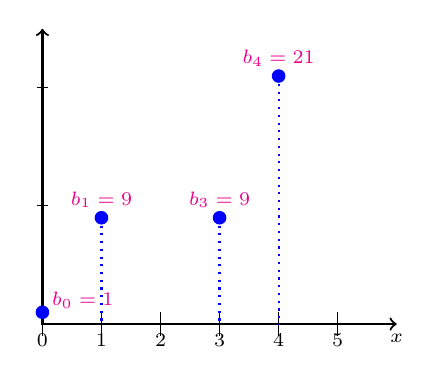
\begin{tikzpicture}[xshift=-4cm,scale=1.5]
\draw[thick,<->] (4,1.5) -- (4,-1) -- (7,-1);
\foreach \x in {4,4.5,...,6.5} \draw (\x,-0.9) -- (\x,-1.1);
\foreach \x in {0,1} \draw (3.95,\x) -- (4.05,\x);
\node[below] at (7,-1) {\scriptsize $x$};
\node[below] at (4,-1) {\scriptsize $0$};
\filldraw[blue] (4,-0.9) circle (1.5pt);
\node[right,magenta] at (4,-0.8) {\scriptsize $b_0=1$};
\node[below] at (4.5,-1) {\scriptsize $1$};
\filldraw[blue] (4.5,-0.1) circle (1.5pt);
\draw[dotted,blue,thick] (4.5,-0.1) -- (4.5,-1);
\node[above,magenta] at (4.5,-0.1) {\scriptsize $b_1=9$};
\node[below] at (5,-1) {\scriptsize $2$};
\node[below] at (5.5,-1) {\scriptsize $3$};
\filldraw[blue] (5.5,-0.1) circle (1.5pt);
\draw[dotted,blue,thick] (5.5,-0.1) -- (5.5,-1);
\node[above,magenta] at (5.5,-0.1) {\scriptsize $b_3=9$};
\node[below] at (6,-1) {\scriptsize $4$};
\filldraw[blue] (6,1.1) circle (1.5pt);
\draw[dotted,blue,thick] (6,1.1) -- (6,-1);
\node[above,magenta] at (6,1.1) {\scriptsize $b_4=21$};
\node[below] at (6.5,-1) {\scriptsize $5$};
\end{tikzpicture}

The above set of equations clearly has no solution as vector $\mathbf{b}$ is not a linear combination of the two column vectors from $\mathbf{A}$: 
\[
\left[\begin{array}{cc} 1&0\\1&1\\1&3\\1&4\end{array}\right]
\left[\begin{array}{c}u_1\\ u_2\end{array}\right]\ne\left[\begin{array}{r}1\\9\\9\\21\end{array}\right]
\]

For example, The line $b = 1 + 8x$ through the first two points is almost certainly not the best line:

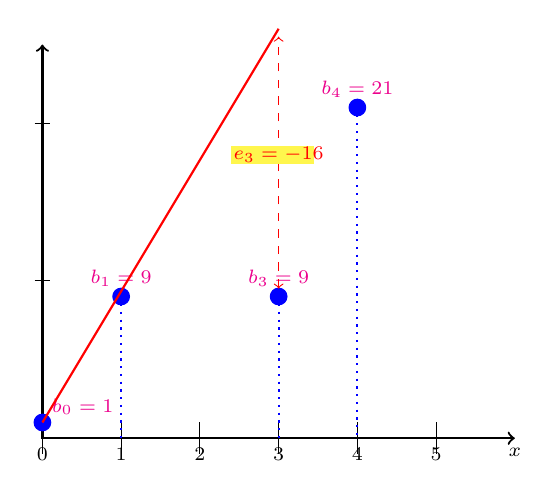
\begin{tikzpicture}[scale=2]
\draw[thick,<->] (0,1.5) -- (0,-1) -- (3,-1);
\foreach \x in {0,0.5,...,2.5} \draw (\x,-0.9) -- (\x,-1.1);
\foreach \x in {0,1} \draw (-0.05,\x) -- (0.05,\x);
\node[below] at (3,-1) {\scriptsize $x$};
\node[below] at (0,-1) {\scriptsize $0$};
\filldraw[blue] (0,-0.9) circle (1.5pt);
\node[right,magenta] at (0,-0.8) {\scriptsize $b_0=1$};
\node[below] at (0.5,-1) {\scriptsize $1$};
\filldraw[blue] (0.5,-0.1) circle (1.5pt);
\draw[dotted,blue,thick] (0.5,-0.1) -- (0.5,-1);
\node[above,magenta] at (0.5,-0.1) {\scriptsize $b_1=9$};
\node[below] at (1,-1) {\scriptsize $2$};
\node[below] at (1.5,-1) {\scriptsize $3$};
\filldraw[blue] (1.5,-0.1) circle (1.5pt);
\draw[dotted,blue,thick] (1.5,-0.1) -- (1.5,-1);
\node[above,magenta] at (1.5,-0.1) {\scriptsize $b_3=9$};
\node[below] at (2,-1) {\scriptsize $4$};
\filldraw[blue] (2,1.1) circle (1.5pt);
\draw[dotted,blue,thick] (2,1.1) -- (2,-1);
\node[above,magenta] at (2,1.1) {\scriptsize $b_4=21$};
\node[below] at (2.5,-1) {\scriptsize $5$};
\draw[red,thick] (0,-0.9) -- (1.5,1.6);
\draw[red,dashed,<->] (1.5,-0.05) -- (1.5,1.55) node[fill,yellow!70] at (1.46,0.8) {~~~~~~~~} node at (1.5,0.8) {\scriptsize $e_3=-16$};
\end{tikzpicture}

But why is this not the best line: look at the {\em error} or {\em residual }, $\mathbf{e}=\mathbf{b}-\mathbf{Au}$.  For the two points the line does not pass through the error is $e_x=b_x-(1+8x)$
is large: $e_3=16$ and $e_4 = 12$.  The {\em Total square error}, $E(\mathbf u) = 0 + 0 + 256 + 144  =400$ .

Notice that the {\em total square error} is given by. 
\[ E(\mathbf u) = \mathbf{e}^{\mathsf{T}}\mathbf{e}\equiv\parallel\mathbf{e}\parallel^2
=(\mathbf{b}-\mathbf{Au})^{\mathsf{T}}(\mathbf{b}-\mathbf{Au})
\]

The Least Squares method  to find the chooses a solution $\mathbf u^*$ that minimises $E(\mathbf u)$.
 
How do we find $\mathbf u^*$?  To find the minimum of $E(\mathbf u)$, we can differentiate with respect to $\mathbf u$, set to 0 and attempt to solve for $\mathbf u$:
\[
\begin{array}{rcl}
 E(\mathbf{u}) &=&(\mathbf{b}-\mathbf{Au})^\mathsf{T}(\mathbf{b}-\mathbf{Au}) \\ \\ 
 &= & \mathbf{b}^\mathsf{T}\mathbf{b} - 2\mathbf{u}^\mathsf{T}\mathbf{A}^\mathsf{T}\mathbf{b}+\mathbf{u}^\mathsf{T} \mathbf{A}^\mathsf{T}\mathbf{A}\mathbf{u}
\end{array}
 \]
 Differentiating and setting to 0:
 \[
 \begin{array}{rrl}
  & \frac{\partial E(\mathbf{u})}{\partial \mathbf{u}} = & 0 \\ \\
\implies  & -2\mathbf{A}^\mathsf{T}\mathbf{b} + 2\mathbf{A}^\mathsf{T}\mathbf{A}\mathbf{u} = & \mathbf{0}\\ \\
\implies  & \mathbf{A}^\mathsf{T}\mathbf{A}\mathbf{u} =& \mathbf{A}^\mathsf{T}\mathbf{b} 
\end{array}
\]
This equation, $\mathbf{A}^\mathsf{T}\mathbf{A}\mathbf{u} = \mathbf{A}^\mathsf{T}\mathbf{b}  $ is called the {\em normal equation}.  

The least squares estimate, $\mathbf{u^*}$, is the solution  to the normal equation.

Notice that $\mathbf A^T \mathbf A$ is square and symmetric.    In some cases it may be possible to directly find the inverse (in particular, when $\mathbf A$ has independent columns, then $\mathbf A^T \mathbf A$ is  positive definite and $\mathbf A^T \mathbf A$ is invertible in which case $\mathbf u^* = ( \mathbf{A}^\mathsf{T}\mathbf{A})^{-1}\mathbf{A}^\mathsf{T}\mathbf{b}$).  In other cases, this approach may be highly unstable, so stable numerical techniques need to be employed.




%%\notinexam{
\subsection{Understanding the Least Squares solution }
\label{sec:leastsqexplain}
{\em This subsection is not examined}.
The main point of this section is to add some geometric and algebraic understanding  to our discussion.  You are not expected to understand all the detail in this section, but do familiarise yourself with the concept and definition of the projection matrix $\mathbf P$ defined below.


The equation $\mathbf{Au} = \mathbf b$ can be seen as  attempting to represent $\mathbf b$   as a linear combination of the $n$ columns of $\mathbf A$.  This is impossible, since the $n$ columns of $\mathbf A$ describe, at most, an $n$-dimensional plane inside the much larger $m$ dimensional space (recall that $n < m$).  Thus $b$ is unlikely to fall on that plane.  The plane is called the {\em column space} of $\mathbf  A$.

\tikz[scale=1.25]{
\draw[fill,yellow!20] (0,0) -- (5,1) -- (6,-1) -- (1,-2) -- cycle;
\draw (0,0) -- (5,1) -- (6,-1) node[left] at (6,-0.7) {\small {\bf column space}} -- (1,-2) -- cycle;
\draw[blue,<->]  (5,0.2) node[above] at (5,0.1) {column $\mathbf{a}_1$} -- (0.8,-0.3) -- (1.2,-1.6) 
node[below] at (1.2,-1.4) {column $\mathbf{a}_n$};
\filldraw (0.8,-0.3) circle (1.5pt); 
\draw[thick] (0.8,-0.3) -- (2,1);
\draw[thick] (0.8,-0.3) -- (2,-1);
\draw[thick,->,dashed] (2,-1) -- (2,0.95) 
node[right] at (1.9,0.2) {\small $\mathbf{e}=\mathbf{b}-\mathbf{Au}^\ast$}
node[right] at (1.9,-0.3) {\scriptsize $\parallel\mathbf{e}\parallel^2 = \parallel\mathbf{b}\parallel^2 - \parallel\mathbf{p}\parallel^2$};
\filldraw[blue] (2,1) circle (1.5pt);
\filldraw[red] (2,-1) circle (1.5pt) node[right] {$\mathbf{p}=\mathbf{Au}^\ast$}; 
\filldraw[yellow!50] (2.2,-2) rectangle (7.5,-1.5);
\draw[thick] (2.2,-2) rectangle (7.5,-1.5); 
\draw (2.2,-1.75) node[right] {\small The best $\mathbf{Au}^\ast$ is the projection $\mathbf{p}$};
}


The best solution, $\mathbf A\mathbf u^* $, is the nearest point to $\mathbf b$ on that plane. Call this point $\mathbf p = \mathbf {Au}^*$.

Now, from a geometric argument, you can see that the error vector $\mathbf e$ is orthogonal (perpendicular) to this plane.  Thus $\mathbf A^T e = 0$.

Notice that  $0 = \mathbf A^T \mathbf e = \mathbf A^T(\mathbf b-\mathbf {Au}^*) = \mathbf A^T\mathbf b - \mathbf A^T\mathbf {Au}^* \implies \mathbf A^T\mathbf b = \mathbf A^T\mathbf{Au}^*$.
This is a geometric derivation of  the normal equation that we earlier saw derived from calculus.  

The point  $\mathbf  p \; (= \mathbf {Au}^*)$ is the projection of $\mathbf b$ onto the column space of $\mathbf A$:
\[
\mathbf{p} = \mathbf{Au}^\ast = 
\underbrace{\left[\mathbf{A}\left(\mathbf{A}^\mathsf{T}\mathbf{A}\right)^{-1}\mathbf{A}^\mathsf{T}\right]}_{\textsf{projection matrix }\mathbf{P}}
\mathbf{b} = \mathbf{Pb},
\]
where we define the {\em Projection matrix}, $\mathbf{P} = \mathbf{A}\left(\mathbf{A}^\mathsf{T}\mathbf{A}\right)^{-1}\mathbf{A}^\mathsf{T}$.  $\mathbf P$ is symmetric and of size $m \times m$ but the rank of $\mathbf P$ is only $n$ (as all the factors of $\mathbf P$ in the definition above have rank $n$).
%%}%end not in exam


\subsection{Computing the Least Squares solution, $\mathbf u^*$ }

We consider three methods for computing the least squares solution to a linear system.  They are Gaussian elimination, QR Decomposition (aka Orthogonalisation) and computation of the pseudo-inverse via SVD.


\subsection{Computing $\mathbf u^*$ via Gaussian elimination}

Given the normal equation $\mathbf A^T\mathbf{Au} = \mathbf A^T\mathbf b$, we may be tempted to find the solution  by Gaussian elimination, where we reduce the the matrix $\mathbf A^T \mathbf A$ to upper triangular form using elementary row operations.

This solution can work but is highly unstable.  To see why it is unstable, consider the condition number of the matrix $\mathbf A^T \mathbf A$.   It can be shown that the condition number of $\mathbf A^T \mathbf A$ is the square of the condition number of $\mathbf A$  (if we take $\sigma_{\min}$ to be the smallest non-zero singular value in the definition of condition number).  So  even if $\mathbf A$ has only moderately widely spread singular values, $\mathbf A^T\mathbf A$  can have a very large condition number and solution by row reduction can be very unstable.




\subsection{Computing $\mathbf u^*$ via orthogonalisation (QR decomposition)}

QR-decompostion presents a much more stable solution to   the normal equation $\mathbf A^\mathrm T\mathbf{Au} = \mathbf A^ \mathrm T\mathbf b$.

The  Orthogonalisation of matrix $\mathbf A$ is given by $\mathbf A = \mathbf {QR}$ where
\begin{itemize}
\item $\mathbf{Q}$ is an $m\times n$ matrix with $n$ orthonormal columns:
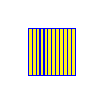
\begin{tikzpicture}
\filldraw[yellow!90] (0,0) -- (0,0.6) -- (0.6,0.6) -- (0.6,0) -- cycle; 
\draw[blue] (0,0) -- (0,0.6) -- (0.6,0.6) --(0.6,0) -- cycle; 
\foreach \x in {0.05,0.1,...,0.6} \draw[blue] (\x,0) -- (\x,0.6);
\end{tikzpicture}.  Construction of $\mathbf Q$ is discussed below.

\item $\mathbf{R }$ is an $n\times n$ upper triangular matrix:

\begin{tikzpicture}
\filldraw[blue] (0.6,0) -- (0,0.6) -- (0.6,0.6) -- cycle; \draw[blue!50] (0,0) -- (0,0.6) -- (0.6,0.6) -- (0.6,0) -- cycle; 
\end{tikzpicture}.  $\mathbf R$ is given by $\mathbf R = \mathbf Q^\mathrm T \mathbf A$.

\end{itemize}


 This factorisation  reduces the normal equation  to a much simpler equation:
\begin{eqnarray*}
\mathbf{A}^\mathsf{T}\mathbf{A}\mathbf{u}&=&\mathbf{A}^\mathsf{T}\mathbf{b}\\
\implies (\mathbf{Q}\mathbf{R})^\mathsf{T}\mathbf{Q}\mathbf{R}\mathbf{u}^\ast &=& (\mathbf{Q}\mathbf{R})^\mathsf{T}\mathbf{b} \\
{\implies}\; \mathbf{R}^\mathsf{T}\mathbf{Q}^\mathsf{T}\mathbf{Q}\mathbf{R}\mathbf{u}^\ast &=&
\mathbf{R}^\mathsf{T}\mathbf{Q}^\mathsf{T}\mathbf{b}
\\
{\implies}\; 
 \mathbf{R}^\mathsf{T} \mathbf{R}\mathbf{u}^\ast &=& \mathbf{R}^\mathsf{T}\mathbf{Q}^\mathsf{T}\mathbf{b} \mbox{ since $\mathbf Q^\mathsf{T}\mathbf Q = \mathbf I $}\\
 {\implies}\; \mathbf{R}\mathbf{u}^\ast  &=& \mathbf{Q}^\mathsf{T}\mathbf{b} \mbox{ multiplying both sides by } (\mathbf{R}^\mathsf{T})^{-1}.
 \end{eqnarray*}
This is easy to solve via back-substitution, since $\mathbf R$ is upper triangular.


\subsubsection{Constructing  the orthogonal matrix $\mathbf Q$ by Gram-Schmidt}

The orthonormal columns of $\mathbf Q$, call them $\mathbf q_1,\ldots, \mathbf q_n$, are obtained iteratively  from the columns $\mathbf{a}_1,\ldots,\mathbf{a}_n$ of $\mathbf{A}$.  The basic idea is that we set $\mathbf q_1$ to be $\mathbf a_1$.  $q_2$ is then set to be $a_2$ and any part of it in the direction of $q_1 (=a_1)$ is subtracted out, so ensure that it is orthogonal to $q_1$.  Similarly, $q_3$ is set to be $a_3$ with any parts in the direction of $q_1$ or $q_2$ are subtracted.  All these vectors are normalised to have magnitude 1 at each step.

This is called the {\em Gram-Schmidt} process and is more formally defined as follows:

\[
\begin{array}{lllll}
\mbox{Set } \mathbf{v}_1&= &  \mathbf{a}_1. &\mbox{ Then} &   \mathbf{q}_1 =  \frac{\mathbf{v}_1}{|\mathbf{v}_1|}. \\ \\
\mbox{Set } \mathbf{v}_2&= & \mathbf{a}_2-\left(\mathbf{a}_2^\mathsf{T}\mathbf{q}_1\right)\mathbf{q}_1. &\mbox{ Then} &   \mathbf{q}_2  =  \frac{\mathbf{v}_2}{|\mathbf{v}_2|}.  \\


\vdots && \vdots && \vdots \hspace{1cm} \vdots \\

\mbox{Set } \mathbf{v}_j &= & \mathbf{a}_j-\sum\limits_{i=1}^{j-1}\left(\mathbf{a}_j^\mathsf{T}\mathbf{q}_i\right)\mathbf{q}_i. &\mbox{ Then} &   \mathbf{q}_j  =  \frac{\mathbf{v}_j}{|\mathbf{v}_j|}.  

\end{array}
\]
Note that  $|\mathbf v|  = \mathbf v^{\mathsf T} \mathbf v$ is the norm of $\mathbf v$.

Having found $\mathbf Q$, find $\mathbf  R$ by setting $\mathbf R = \mathbf{Q^\top A}$.  $\mathbf R$ is indeed upper triangular since the $i$th column of $\mathbf Q$ is, by construction, orthogonal to first $i-1$ columns of $\mathbf A$.

Producing $\mathbf{Q}$ and $\mathbf{R}$ takes twice as long as the 
$mn^2$ steps to form $\mathbf{A}^\mathsf{T}\mathbf{A}$, but that extra cost gives a more reliable solution.

There is another method of orthogonalisation that we don't cover here  which has  better numerical stability using so-called Householder reflectors.  

{\bf Example:} Use the Gram-Schmidt process to orthogonalise the matrix 
\[ \mathbf{A}=\left[\begin{array}{ccc}1&0&0\\1&0&1\\1&1&0\\1&1&1\end{array}\right]. \]

{\bf Solution}: 
Let $ \mathbf{v}_1 = \mathbf{a}_1 = 
 \left[\begin{array}{c}1\\1\\1\\1\end{array}\right] $ and then normalise to get 
$ \mathbf{q}_1 =   \frac{ \mathbf{v}_1 }{ | \mathbf{v}_1 | } = \left[\begin{array}{c}0.5\\0.5\\0.5\\0.5\end{array}\right]$. 
Now set $ \mathbf{v}_2 = \mathbf a_2  - (\mathbf a_2^\top \mathbf q_1)\mathbf q_1  = \left[ \begin{array}{c}0\\0\\1\\1\end{array} \right] -
\left(
       \left[ \begin{array}{cccc}0&0&1&1\end{array}\right] 
       \left[ \begin{array}{c}0.5\\0.5\\0.5\\0.5\end{array} \right]
\right) \left[ \begin{array}{c}0.5\\0.5\\0.5\\0.5\end{array} \right] = \left[ \begin{array}{r}-0.5\\-0.5\\0.5\\0.5\end{array} \right] $.  Since $\mathbf v_2 = 1$, $\mathbf q_2 = \frac{\mathbf v_2}{| \mathbf v_2|} = \mathbf v_2$.

Finally, to get $\mathbf q_3$, set 

\begin{align*}
\mathbf v_3 & =   \mathbf a_3  - (\mathbf a_3^\top \mathbf q_1)\mathbf q_1 - (\mathbf a_3^\top \mathbf q_2)\mathbf q_2  \\ 
  &=  \left[ \begin{array}{c}0\\1\\0\\1\end{array} \right] -
\left(
       \left[ \begin{array}{cccc}0&1&0&1\end{array}\right] 
       \left[ \begin{array}{c}0.5\\0.5\\0.5\\0.5\end{array} \right]
\right) \left[ \begin{array}{c}0.5\\0.5\\0.5\\0.5\end{array} \right] 
- \left(
       \left[ \begin{array}{cccc}0&1&0&1\end{array}\right] 
       \left[ \begin{array}{r}-0.5\\-0.5\\0.5\\0.5\end{array} \right]
\right) \left[ \begin{array}{r}-0.5\\-0.5\\0.5\\0.5\end{array} \right] \\
  &= 
\left[ \begin{array}{r}0.5\\-0.5\\0.5\\-0.5\end{array} \right] 
\end{align*}
which is also normalised, so $\mathbf q_3 = \mathbf v_3$ and 
\[ 
\mathbf Q = \frac{1}{2}
 \left[ \begin{array}{rrr}1&-1&1\\1&-1&-1\\1&1&1\\1&1&-1\end{array}\right].
\]
We find $\mathbf R$ as follows:
\[ \mathbf{R}=\mathbf{Q}^\mathsf{T}\mathbf{A}
= \frac{1}{2}\left[\begin{array}{rrrr}1&1&1&1\\-1&-1&1&1\\1&-1&1&-1\end{array}\right]
\left[ \begin{array}{rrr}1&0&0\\1&0&1\\1&1&0\\1&1&1\end{array}\right] = 
\left[ \begin{array}{rrr}2&1&1\\ 0&1& 0\\ 0&0&-1\end{array}\right]. 
\] \sqend




\subsection{Computing $\mathbf u^*$ via SVD: the Pseudoinverse}

The most stable computation to find the solution to the normal equation is given by singular value decomposition (SVD).

Recall that SVD decomposes the $m \times n$ matrix $\mathbf  A$ as $\mathbf{A}= \mathbf{UDV}^\mathsf{T}$ where:

\begin{itemize}
\item $\mathbf{U}$ is a column-orthonormal $n\times m$ matrix, so $\mathbf{U}^\mathsf{T}\mathbf{U}=\mathbf{I}_n$,
\item $\mathbf{V}$ is an orthonormal $n\times n$ matrix so 
$\mathbf{V}^\mathsf{T}\mathbf{V}=\mathbf{I}_n$ (indeed, $\mathbf V ^ \mathrm T = \mathbf V ^ {-1} $), and 

\item $\mathbf{D}=\mathrm{diag}\{\sigma_1,\ldots,\sigma_n\}$ is a diagonal $n\times n$ matrix of singular values.  Since $\mathbf{D}$ is diagonal, $\mathbf{D}^\mathsf{T}=\mathbf{D}$.
\end{itemize}

Now consider the product $\mathbf{A}^\mathsf{T}\mathbf{A} $ that arises in the normal equation.  Substituting $\mathbf{A}= \mathbf{UDV}^\mathrm{T}$ in this product gives:
\[ 
\mathbf{A}^\mathsf{T}\mathbf{A} = ({\mathbf{UDV}^\mathsf{T}})^\mathsf{T}\mathbf{UDV}^\mathsf{T}=  \mathbf{VD}^\mathsf{T}\mathbf{U}^\mathsf{T}\mathbf{UDV}^\mathsf{T}
  = \mathbf{VD}^\mathsf{T}\mathbf{DV}^\mathsf{T} =  \mathbf{VD}^2\mathbf{V}^\mathsf{T}.
\]
We can thus express  the normal equation in a much simplified form:
\begin{eqnarray*}
\mathbf{A}^\mathsf{T}\mathbf{A}\mathbf{u}&=&\mathbf{A}^\mathsf{T}\mathbf{b}\\
\implies \mathbf{V}{\mathbf{D}^2\mathbf{V}^\mathsf{T}\mathbf{u}^\ast} &=& \mathbf{V}{\mathbf{D}\mathbf{U}^\mathsf{T}\mathbf{b}}\\
\implies \mathbf{D}^2\mathbf{V}^\mathsf{T}\mathbf{u}^\ast &=&   
\mathbf{D}\mathbf{U}^\mathsf{T}\mathbf{b} \\
\implies \mathbf{V}^\mathsf{T}\mathbf{u}^\ast &=&
\underbrace{\left(\mathbf{D}^2\right)^{-1}\mathbf{D}}_{\mathbf{D}^{+}}
\mathbf{U}^\mathsf{T}\mathbf{b}\\
\implies \mathbf{u}^\ast &=& \mathbf{V}\mathbf{D}^{+}\mathbf{U}^\mathsf{T}\mathbf{b}.
 \end{eqnarray*}
The matrix $\mathbf{D}^{+}$ is called the ``{\em pseudoinverse}" of $\mathbf{D}$ and is defined as follows:
$\mathbf{D}^{+}=\mathrm{diag}\left\{\sigma^{+}_1,\ldots,\sigma^{+}_n\right\}$ where
\[
\sigma^{+}_i =\left\{\begin{array}{lll}\sigma_i^{-1}=\frac{1}{\sigma_i}&\mathsf{if}& \sigma_i > 0\\
0 &\multicolumn{2}{l}{\textsf{otherwise.}}
\end{array}\right.
\]
Thus if $\mathrm{rank}(\mathbf{A}) = n$, then all the singular values of $\mathbf A$ are non-zero, in which case $\mathbf D^{+} = \mathbf D^{-1} = \mathrm{diag}\left\{\frac 1 {\sigma_1},\ldots,\frac 1 {\sigma_n} \right\}$.  In this case, In the former case, $\mathbf{DD}^+ = \mathbf D^+ \mathbf D = \mathbf I_n$.   

However, if $\mathrm{rank}(\mathbf{A}) = r < n$, there are only $r < n$ non-zero singular values and $\mathbf D^{+} = \mathrm{diag}\{\frac 1 {\sigma_1},\ldots,\frac 1 {\sigma_k}, \underbrace{0,\ldots,0}_{n-r \mbox{ zeros}}\}.$   In this case, $\mathbf{DD}^+ = \mathbf D^+ \mathbf D = \mathrm{diag}\{1,\ldots,1 , \underbrace{0,\ldots,0}_{n-r \mbox{ zeros}}\}$ --- which is very close to, but not quite, the identity matrix.


We call the product matrix $ \mathbf{V}\mathbf{D}^{+}\mathbf{U}^\mathsf{T}$ the  {\em pseudoinverse} of $\mathbf A$, written $\mathbf A^+$.  That is ,
\[
\mathbf{A}^{+} = \mathbf{V}\mathbf{D}^{+}\mathbf{U}^\mathsf{T}.
\]
If $\mathrm {rank}(\mathbf A) = n$, then  $
  \mathbf{A}^+\mathbf{A} = 
  \mathbf{V}{\mathbf{D}^{+}{\mathbf{U}^\mathsf{T}\mathbf{U}}\mathbf{D}}\mathbf{V}^\mathsf{T}  = \mathbf{V}{\mathbf{D}^{+}\mathbf{D}}\mathbf{V}^\mathsf{T} = \mathbf{V}\mathbf{V}^\mathsf{T} = \mathbf{I}_n$, and $\mathbf A^+ = \mathbf A^{-1}$.
 
 
Recall  that the matrix $\mathbf A^ \mathrm T \mathbf A$ is ill-conditioned when the smallest singular value, $\sigma_n$, is very small.  This leads to  instability in computing the solution to the normal equation.  The pseudo-inverse method provides a way of removing this instability to get an approximate but stable solution by simply removing the smallest singular value or values.  
 
 
 
 \subsubsection{Properties of the pseudo inverse $\mathbf A^+$}

The pseudo-inverse of $\mathbf A$ always exists (all we need to do is calculate the SVD and form the product described above).
 
 The SVD of $\mathbf A$ gives $ \mathbf{A} = \mathbf{UDV}^\mathsf{T}$ from which we get  $\mathbf{AV} = \mathbf{UD}$ or, considering the individual columns,  
$\mathbf{Av}_i = \sigma_i\mathbf{u}_i$.
\begin{itemize}
\item If $\mathbf{A}$ is a square matrix such that $\mathbf{A}^{-1}$ exists, then the singular values for 
$\mathbf{A}^{-1}$ are $\sigma^{-1}=\frac{1}{\sigma}$  and $\mathbf{A}^{-1}\mathbf{u}_i =\frac{1}{\sigma_i}\mathbf{v}_i$ 
\item If $\mathbf{A}^{-1}$  does not exist, then the {pseudoinverse} matrix $\mathbf{A}^{+}$ does exist such that: 
\[
\mathbf{A}^{+}\mathbf{u}_i =\left\{\begin{array}{lll}
 \frac{1}{\sigma_i}\mathbf{v}_i & \textsf{if}  & i \le r = \mathrm{rank}(\mathbf{A}) \textsf{  i.e. if   } \sigma_i > 0\\
 0                                                  & \textsf{for} & i > r.
 \end{array}
\right.
\]
\item Pseudoinverse matrix $\mathbf{A}^{+}$ has the same rank $r$ as $\mathbf{A}$
\item The matrices $\mathbf{AA}^{+}$  and $\mathbf{A}^{+}\mathbf{A}$  are also as near as possible to the $m\times m$ and $n\times n$  identity matrices, respectively
\item $\mathbf{AA}^{+}$ -- the $m\times m$ projection matrix onto the column space of $\mathbf{A}$
\item $\mathbf{A}^{+}\mathbf{A}$ -- the $n\times n$ projection matrix onto the row space of $\mathbf{A}$
\end{itemize}


{\bf Example:} Find the pseudo-inverse of  $\mathbf{A}=\left[\begin{array}{cc}0&1\\1&1\\1&0\end{array}\right].$

{\bf Solution:} The singular value decomposition of $\mathbf A$ is 
\[
\mathbf{A}= \mathbf{UDV^\top} =
\underbrace{\left[\begin{array}{rr}
\frac{1}{\sqrt{6}}\vspace*{1mm}&\frac{1}{\sqrt{2}}\\\frac{2}{\sqrt{6}}\vspace*{1mm}&0\\ \frac{1}{\sqrt{6}}&-\frac{1}{\sqrt{2}} 
\end{array}\right]}_{\mathbf{U}}
\underbrace{\left[\begin{array}{rr}
\sqrt{3}&0\\0&1
\end{array}\right]}_{\mathbf{D}}
\underbrace{\left[\begin{array}{rr}
\frac{1}{\sqrt{2}}&\frac{1}{\sqrt{2}}\\-\frac{1}{\sqrt{2}}&\frac{1}{\sqrt{2}}
\end{array}\right]}_{\mathbf{V}^\mathsf{T}}.
\]
So the pseudo-inverse of $\mathbf A$ is 
\begin{align*}
\mathbf{A}^{+}= \mathbf{VD^+U^\top} & = 
\underbrace{\left[\begin{array}{rr}
\frac{1}{\sqrt{2}}\vspace*{1mm}&-\frac{1}{\sqrt{2}}\\ \frac{1}{\sqrt{2}}&\frac{1}{\sqrt{2}}
\end{array}\right]}_{\mathbf{V}}
\underbrace{\left[\begin{array}{rr}
\frac{1}{\sqrt{3}}&0\\0&1
\end{array}\right]}_{\mathbf{D}^{+}}
\underbrace{\left[\begin{array}{rrr}
\frac{1}{\sqrt{6}}\vspace*{1mm}&\frac{2}{\sqrt{6}}& \frac{1}{\sqrt{6}}\\
\frac{1}{\sqrt{2}} &0 &-\frac{1}{\sqrt{2}} 
\end{array}\right]}_{\mathbf{U}^\mathsf{T}} \\
&= \left[\begin{array}{rrr}
-\frac{1}{3}&\frac{1}{3}& \frac{2}{3}\\
\frac{2}{3} &\frac{1}{3} &-\frac{1}{3} 
\end{array}\right].
\end{align*}
Now let's check the products $\mathbf{AA^+}$ and $\mathbf{A^+A}$:
\[
\mathbf{A}\mathbf{A}^{+}=
\left[\begin{array}{cc}0&1\\1&1\\1&0\end{array}\right] 
\left[\begin{array}{rrr}
-\frac{1}{3}\vspace*{1mm}&\frac{1}{3}& \frac{2}{3}\\
\frac{2}{3} &\frac{1}{3} &-\frac{1}{3} 
\end{array}\right]
=
\left[\begin{array}{rrr}
\frac{2}{3}\vspace*{1mm}&\frac{1}{3}& -\frac{1}{3}\\
\frac{1}{3}\vspace*{1mm}&\frac{2}{3}& \frac{1}{3}\\
-\frac{1}{3} &\frac{1}{3} &\frac{2}{3} 
\end{array}\right]
\]
while 
\[
\mathbf{A}^{+}\mathbf{A}=
\left[\begin{array}{rrr}
-\frac{1}{3}\vspace*{1mm}&\frac{1}{3}& \frac{2}{3}\\
\frac{2}{3} &\frac{1}{3} &-\frac{1}{3} 
\end{array}\right]
\left[\begin{array}{cc}0&1\\1&1\\1&0\end{array}\right] 
=
\left[\begin{array}{cc}1&0\\0&1\end{array}\right].
\] \sqend


We end our discussion on computational methods in linear algebra here.  We have only touched on a small number of the wide variety of techniques used in this area, but we have tried to direct our attention to some of the more common and useful techniques.  This is a rich and extremely useful area of study and we encourage interested students to look into fields where these tools and ideas are applied and explored further including computer vision,  engineering, physics, applied mathematics and statistics.
